

\subsection{Training Behaviour}

Figure~\ref{fig:results_training_history} shows a representative \(3e\)
Transformer training run. The first displayed point follows one complete epoch
of optimisation, rather than representing the untrained model.

\begin{figure}[htbp]
    \centering
    \begin{minipage}[t]{0.49\textwidth}
        \centering
        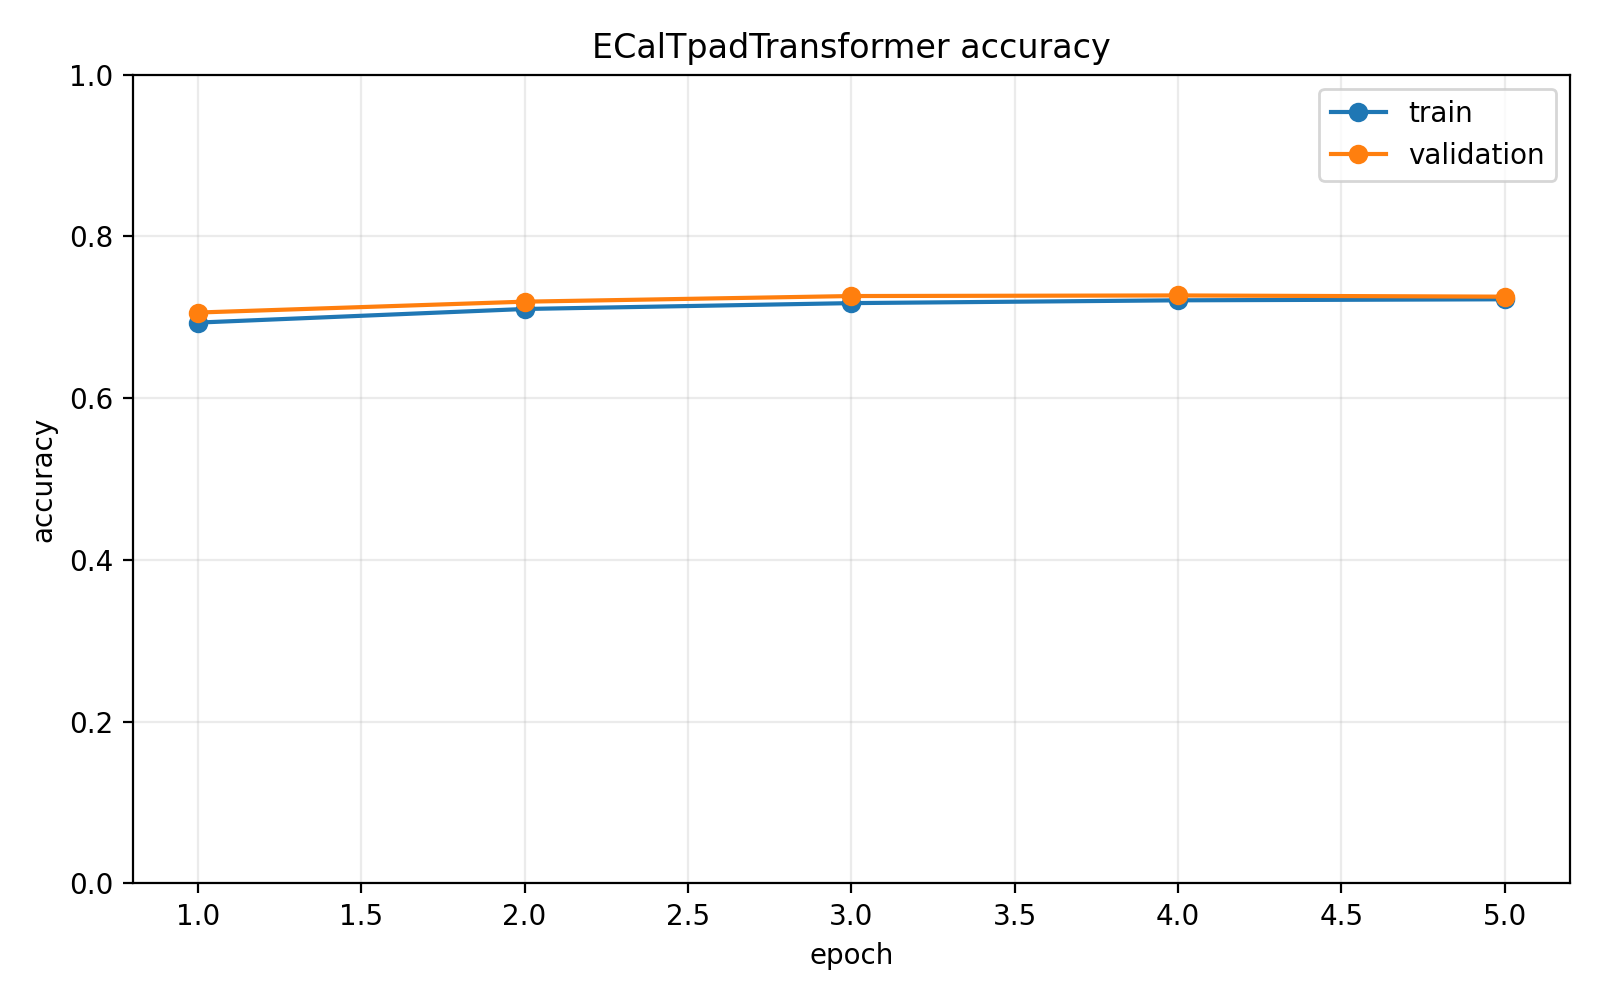
\includegraphics[width=\linewidth]{config/fig/results/training_accuracy_3e.png}
    \end{minipage}\hfill
    \begin{minipage}[t]{0.49\textwidth}
        \centering
        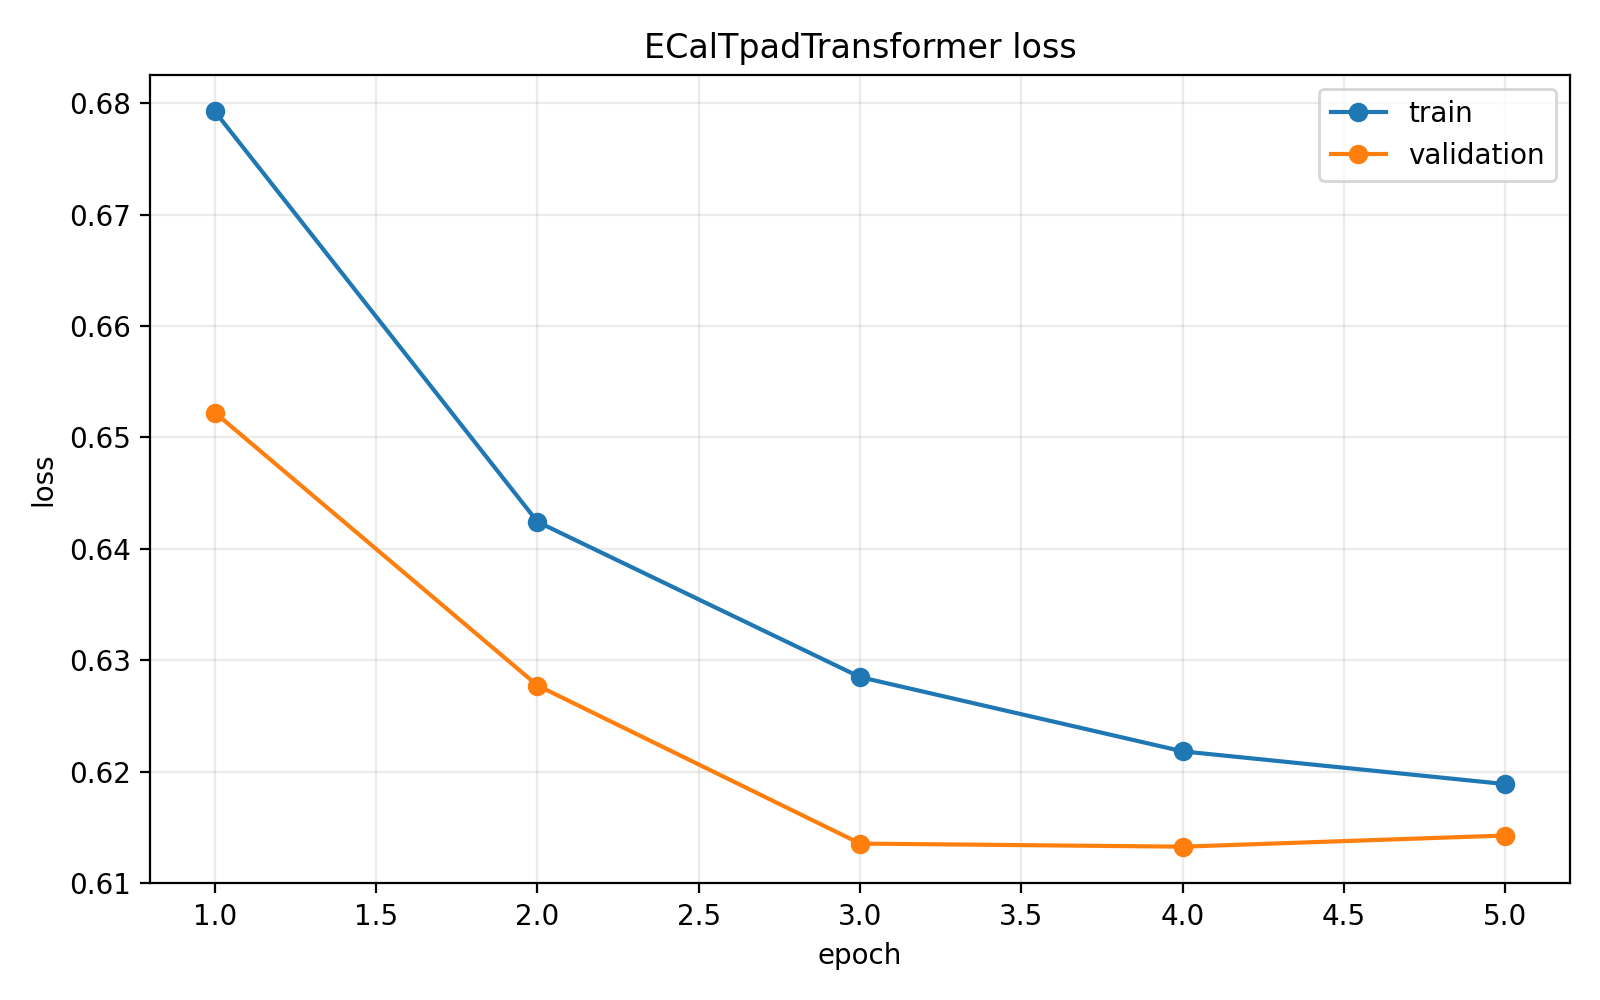
\includegraphics[width=\linewidth]{config/fig/results/training_loss_3e.png}
    \end{minipage}
    \caption{Training history for a representative \(3e\)
    \texttt{ECalTpadTransformer} development run using \(16{,}000\) training
    and \(3{,}000\) validation events. The left panel shows native-label hit
    accuracy and the right panel shows cross-entropy loss.}
    \label{fig:results_training_history}
\end{figure}

The training accuracy increases from \(0.693\) after the first epoch to
\(0.722\) after the fifth, while the validation accuracy changes from \(0.706\)
to \(0.726\). Over the same interval, the training loss decreases from
\(0.679\) to \(0.619\), and the validation loss reaches its minimum of
\(0.613\) after epoch four before increasing slightly. The continuing loss
reduction with only a small change in accuracy means that the predicted class
probabilities are still changing even when relatively few maximum-probability
assignments change. The rapid plateau suggests that additional epochs alone
are unlikely to produce a large improvement for this configuration. It does
not establish that additional training events are unnecessary, which would
require a dedicated learning-curve study.

\clearpage
\subsection{Hit and Event Assignment Performance}

The event-wise distributions in Figure~\ref{fig:results_event_accuracy}
show that reconstruction quality varies substantially between events. The
median permutation-aligned event hit accuracy is \(0.854\) for \(2e\) and
\(0.757\) for \(3e\) events. The corresponding event means are \(0.829\) and
\(0.744\), while the pooled hit accuracies are \(0.833\) and \(0.748\).
The additional electron therefore makes the assignment task more difficult,
but the broad distributions also show that electron multiplicity alone does
not determine whether an event is reconstructed well.

\begin{figure}[htbp]
    \centering
    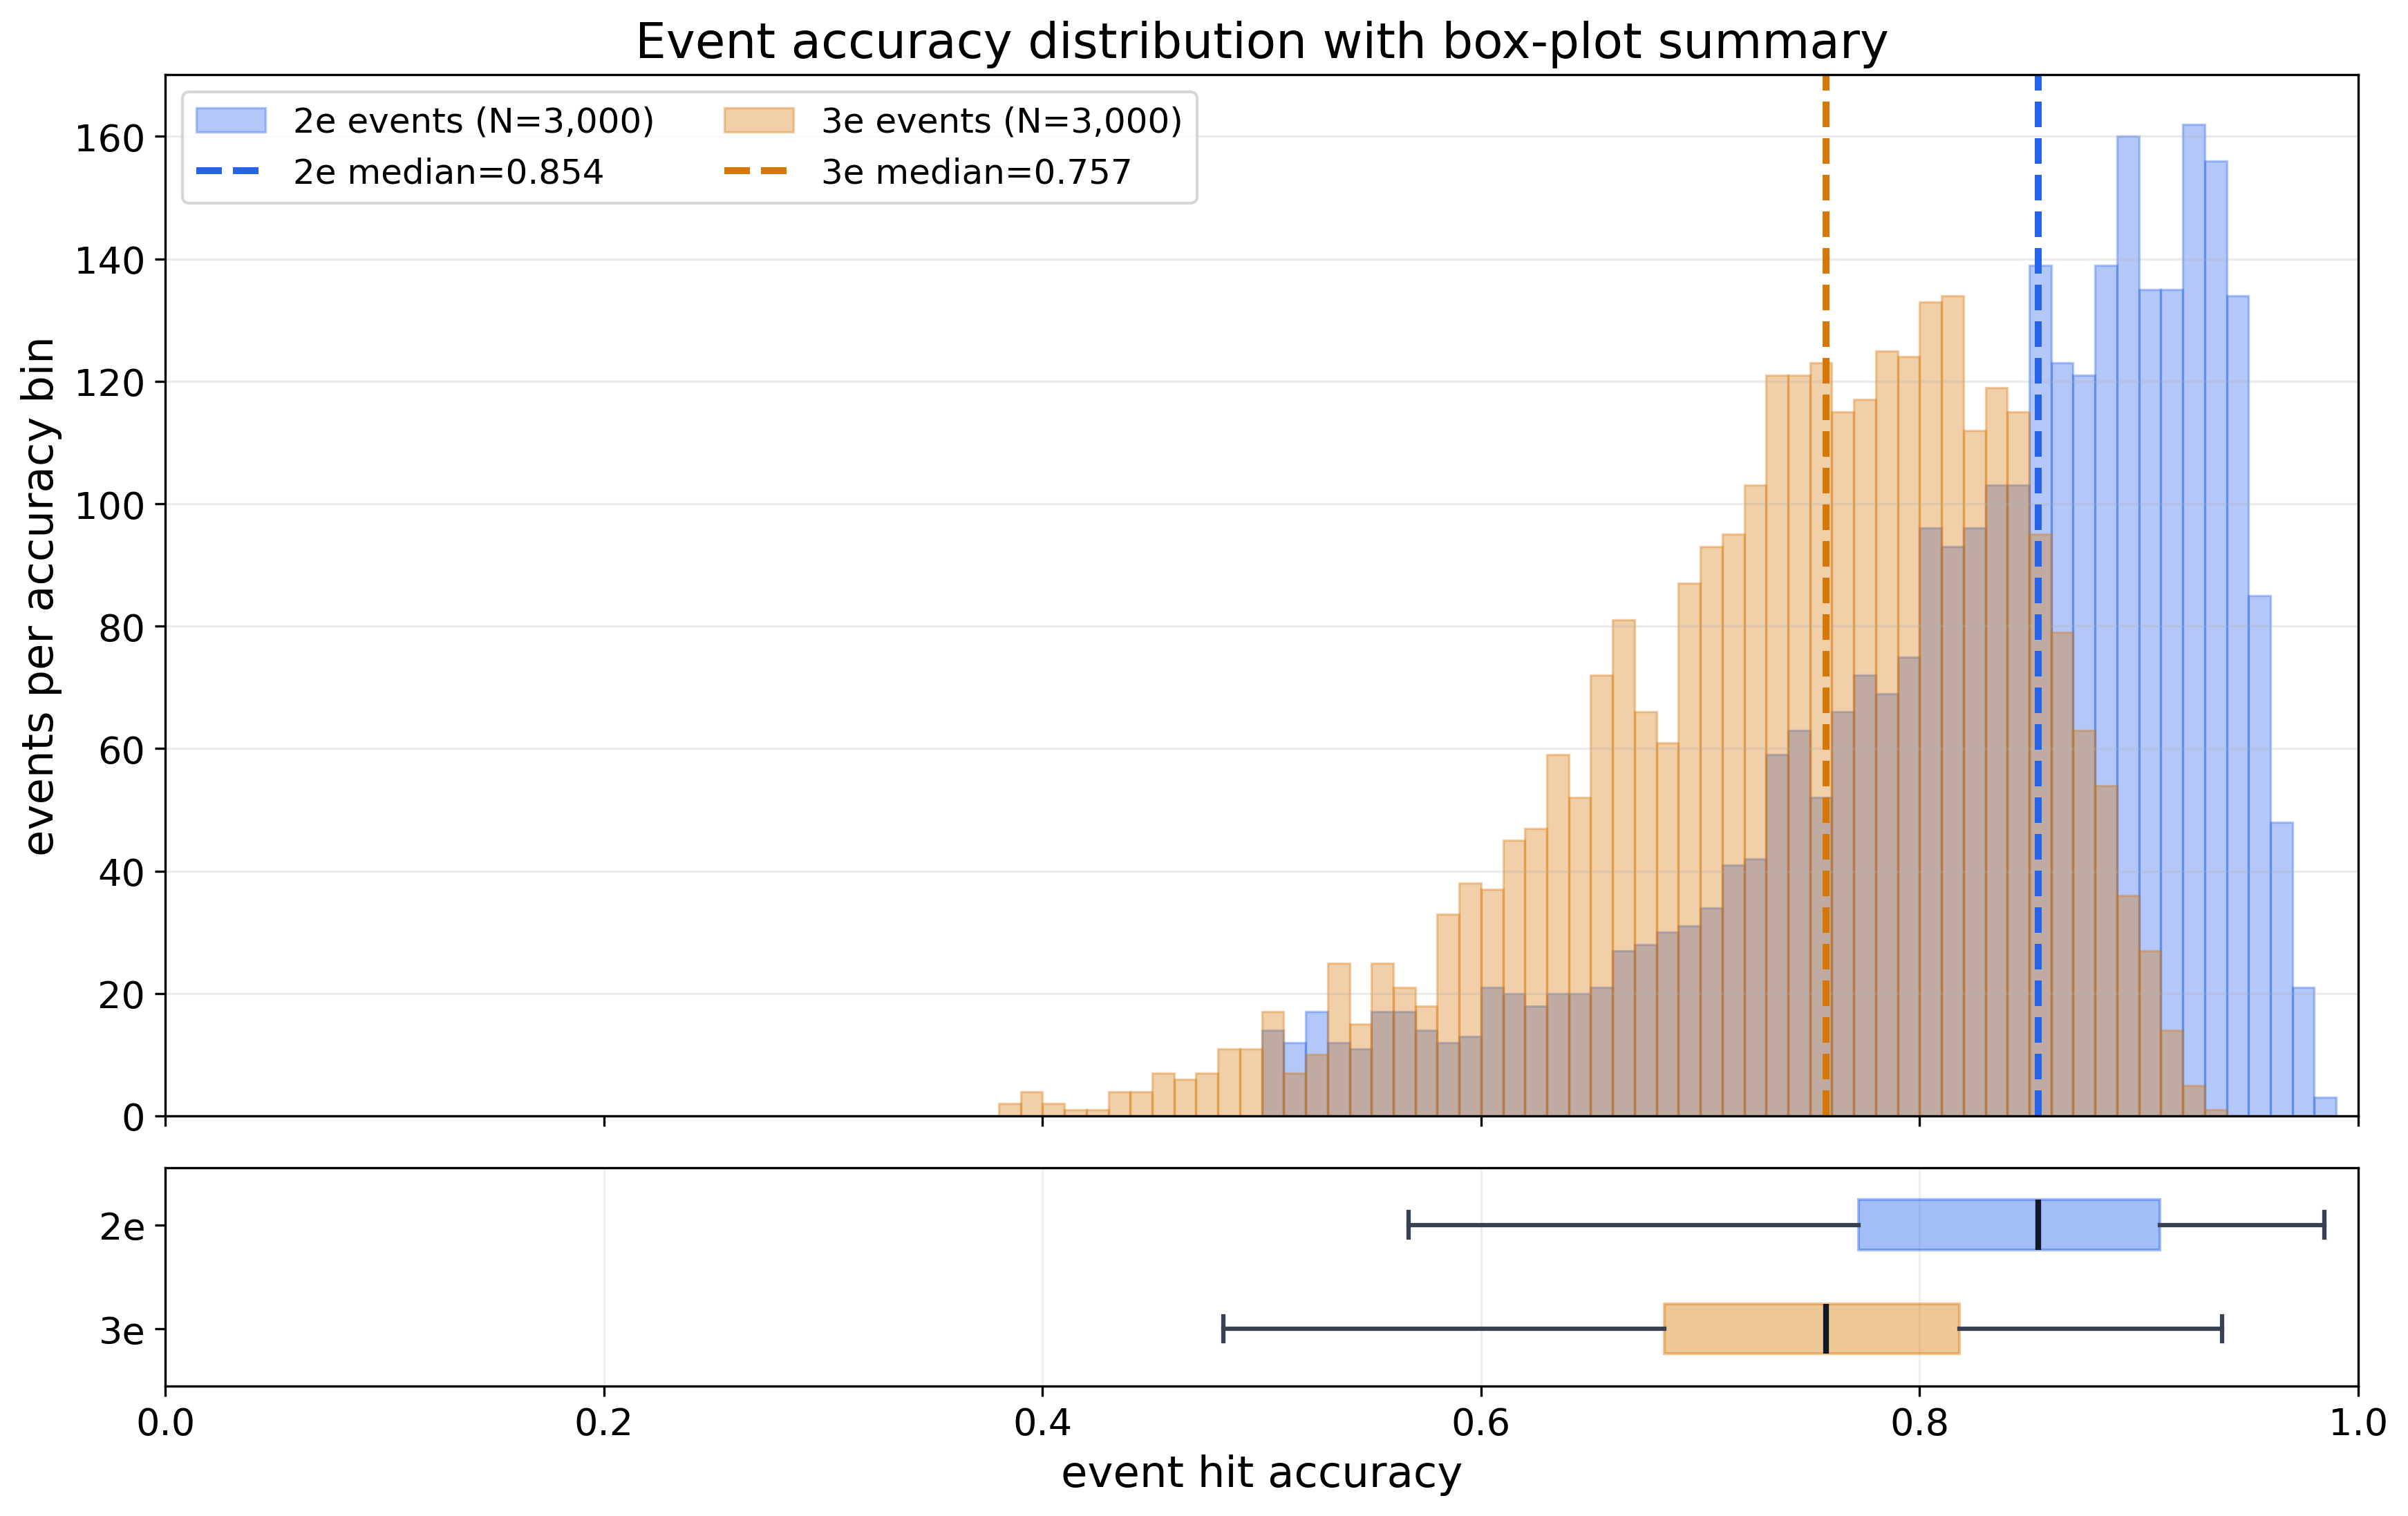
\includegraphics[width=0.98\linewidth]{config/fig/results/event_accuracy_distribution.png}
    \caption{Distribution of permutation-aligned event hit accuracy for
    \(3{,}000\) \(2e\) and \(3{,}000\) \(3e\) validation events. Every event
    contributes equally to the histogram and box-plot summary. Dashed lines
    indicate the sample medians.}
    \label{fig:results_event_accuracy}
\end{figure}

Figure~\ref{fig:results_confusion} separates the same result by true and
predicted electron group. For \(2e\), the two groups have similar overall
recall. For \(3e\), the middle canonical group is confused more frequently
with both neighbouring groups than either outer group. The decrease in the
last twelve ECal layers is visible for both multiplicities: pooled accuracy is
\(0.693\) for \(2e\) and \(0.556\) for \(3e\), compared with \(0.836\) and
\(0.751\) in layers 1--20. The last-layer group contains only about \(1.5\,\%\)
of the hits in each sample and should not be given the same statistical weight
as the all-layer result.

\begin{figure}[htbp]
    \centering
    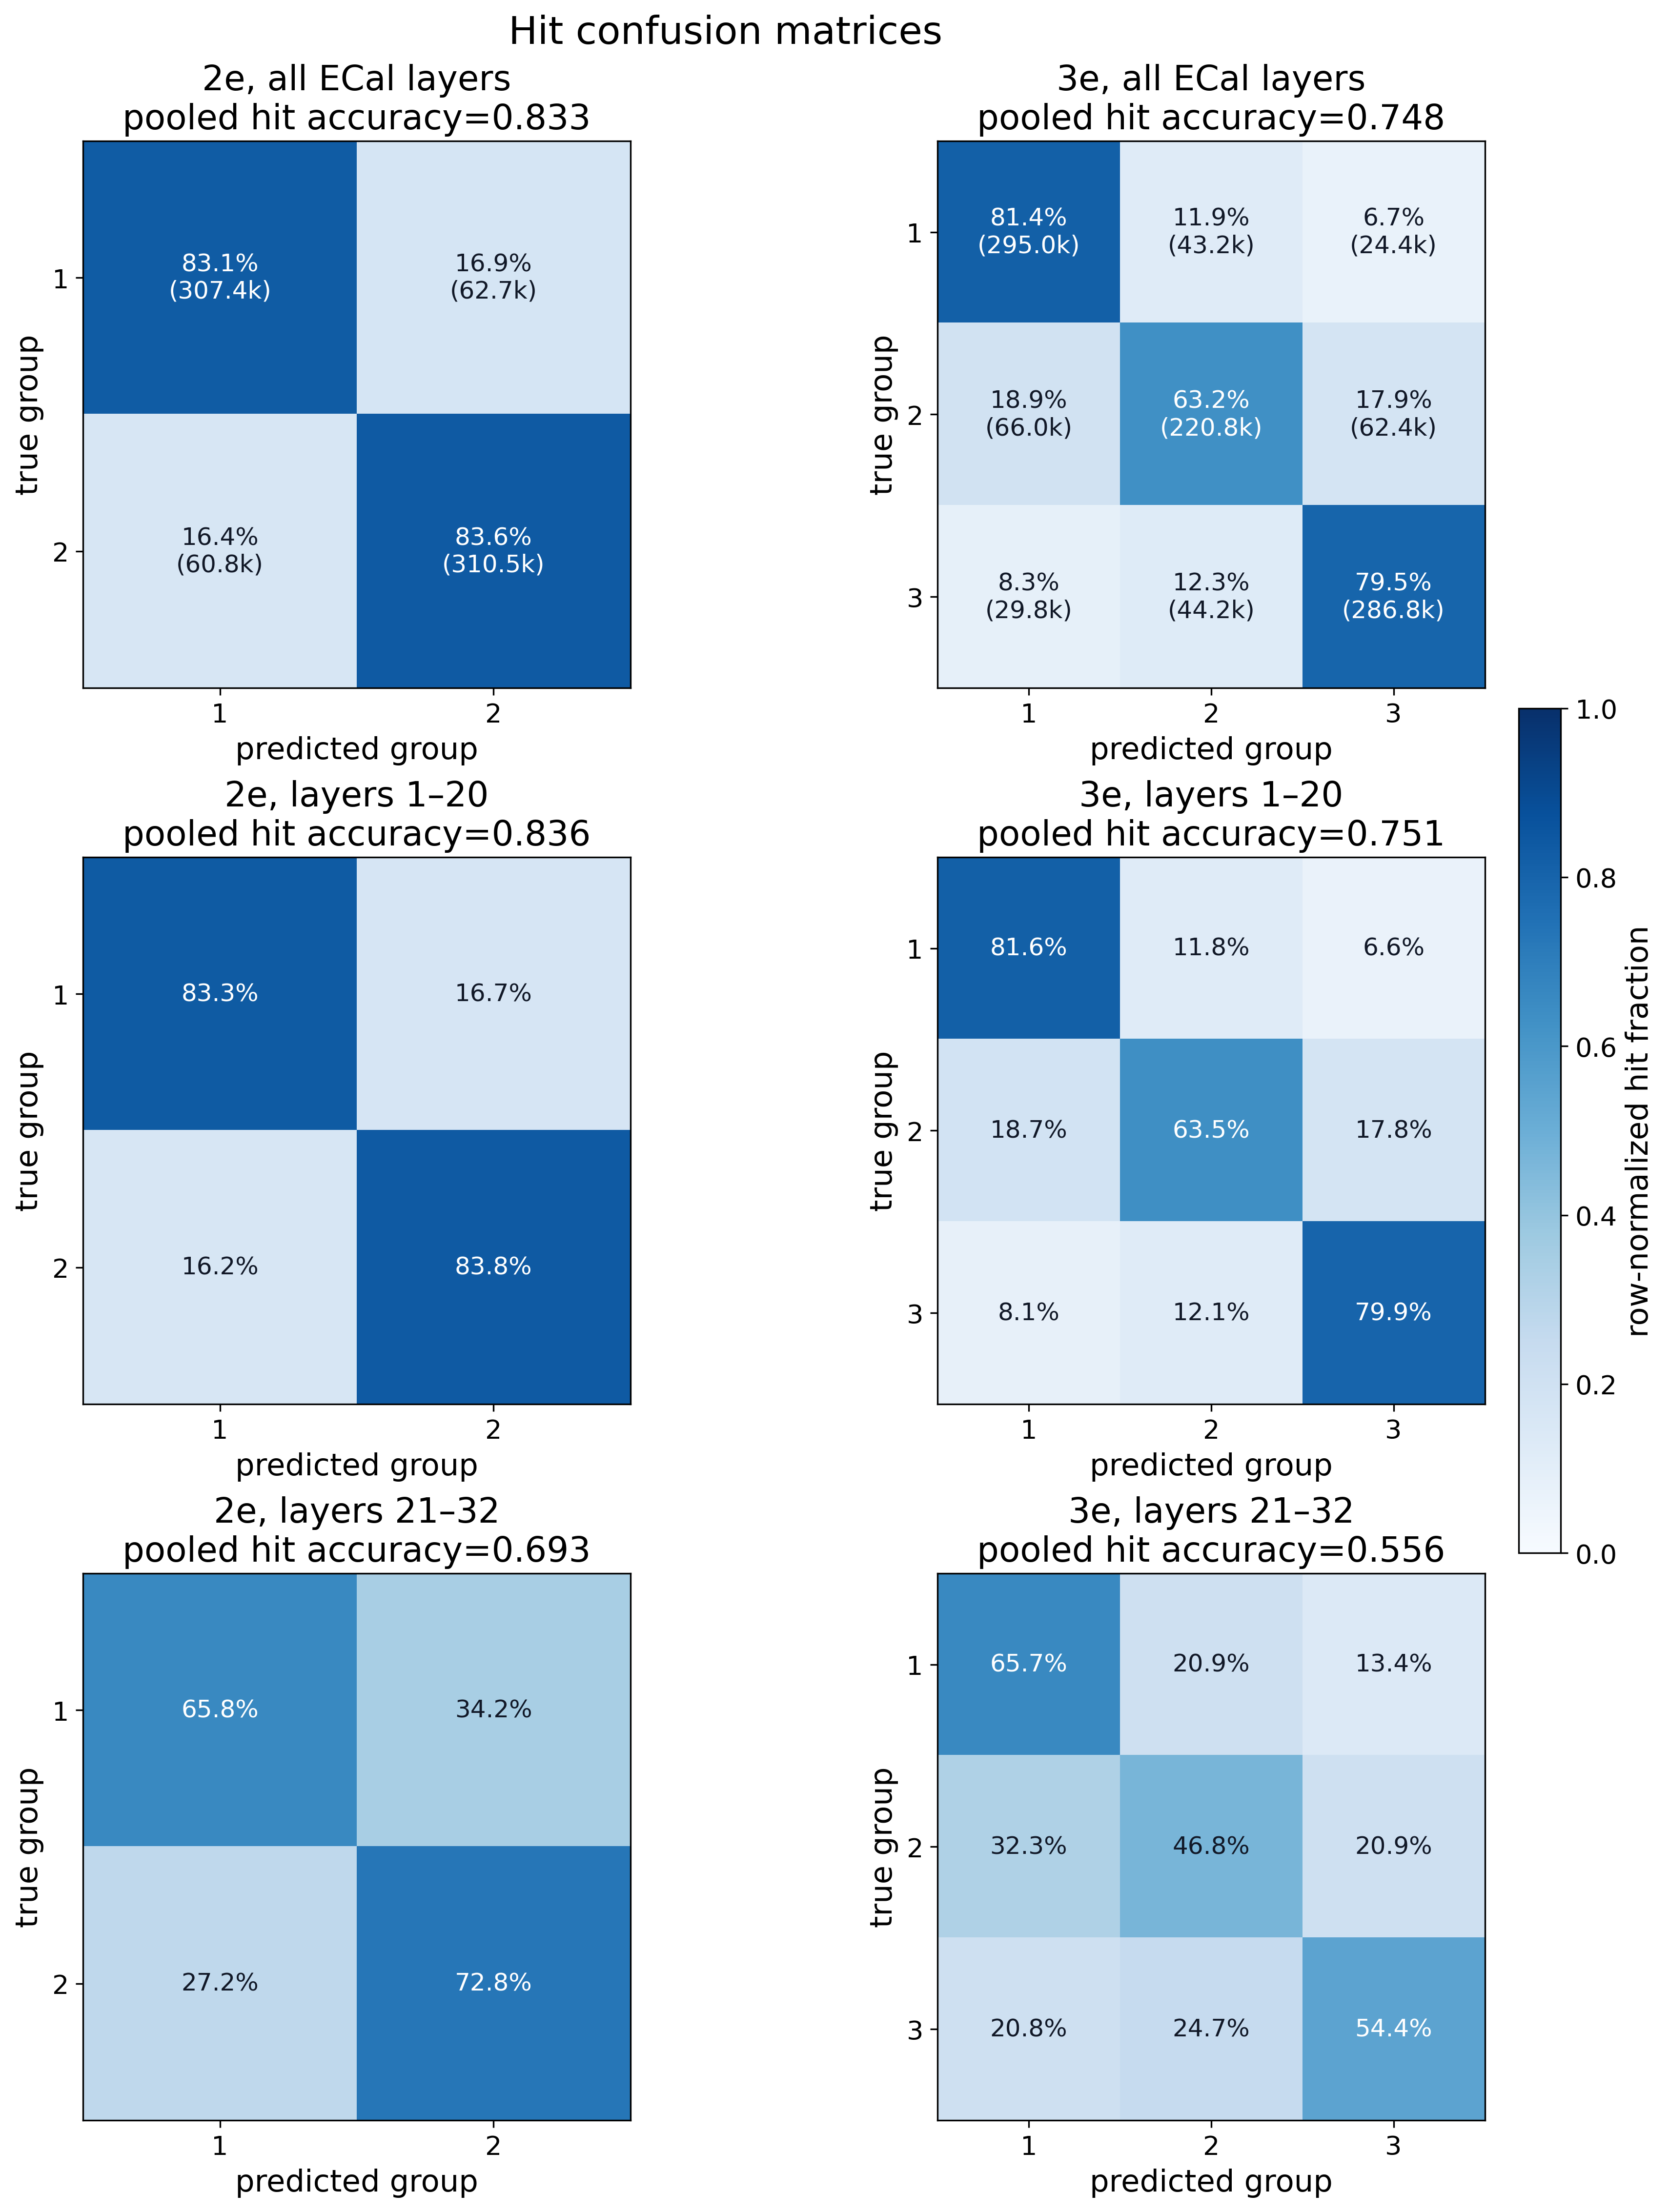
\includegraphics[height=0.76\textheight,keepaspectratio]{config/fig/results/hit_confusion_matrices.png}
    \caption{Row-normalized hit confusion matrices after one event-wide label
    alignment. Rows are true groups and columns are predicted groups. The top
    row uses all ECal layers, the middle row uses layers 1--20 and the bottom
    row uses layers 21--32. Percentages are conditional on the true group, and
    counts are pooled over validation hits.}
    \label{fig:results_confusion}
\end{figure}

\clearpage
\subsection{Performance Across the ECal Depth}

Figures~\ref{fig:results_layer_hit_accuracy}
and~\ref{fig:results_layer_energy_accuracy} resolve the assignment performance
layer by layer. The mean hit accuracy decreases with ECal depth for both event
multiplicities, with the \(3e\) sample remaining below the \(2e\) sample. The
late-layer fluctuations and confidence intervals should be interpreted
cautiously because relatively few event-layer observations remain there.

\begin{figure}[htbp]
    \centering
    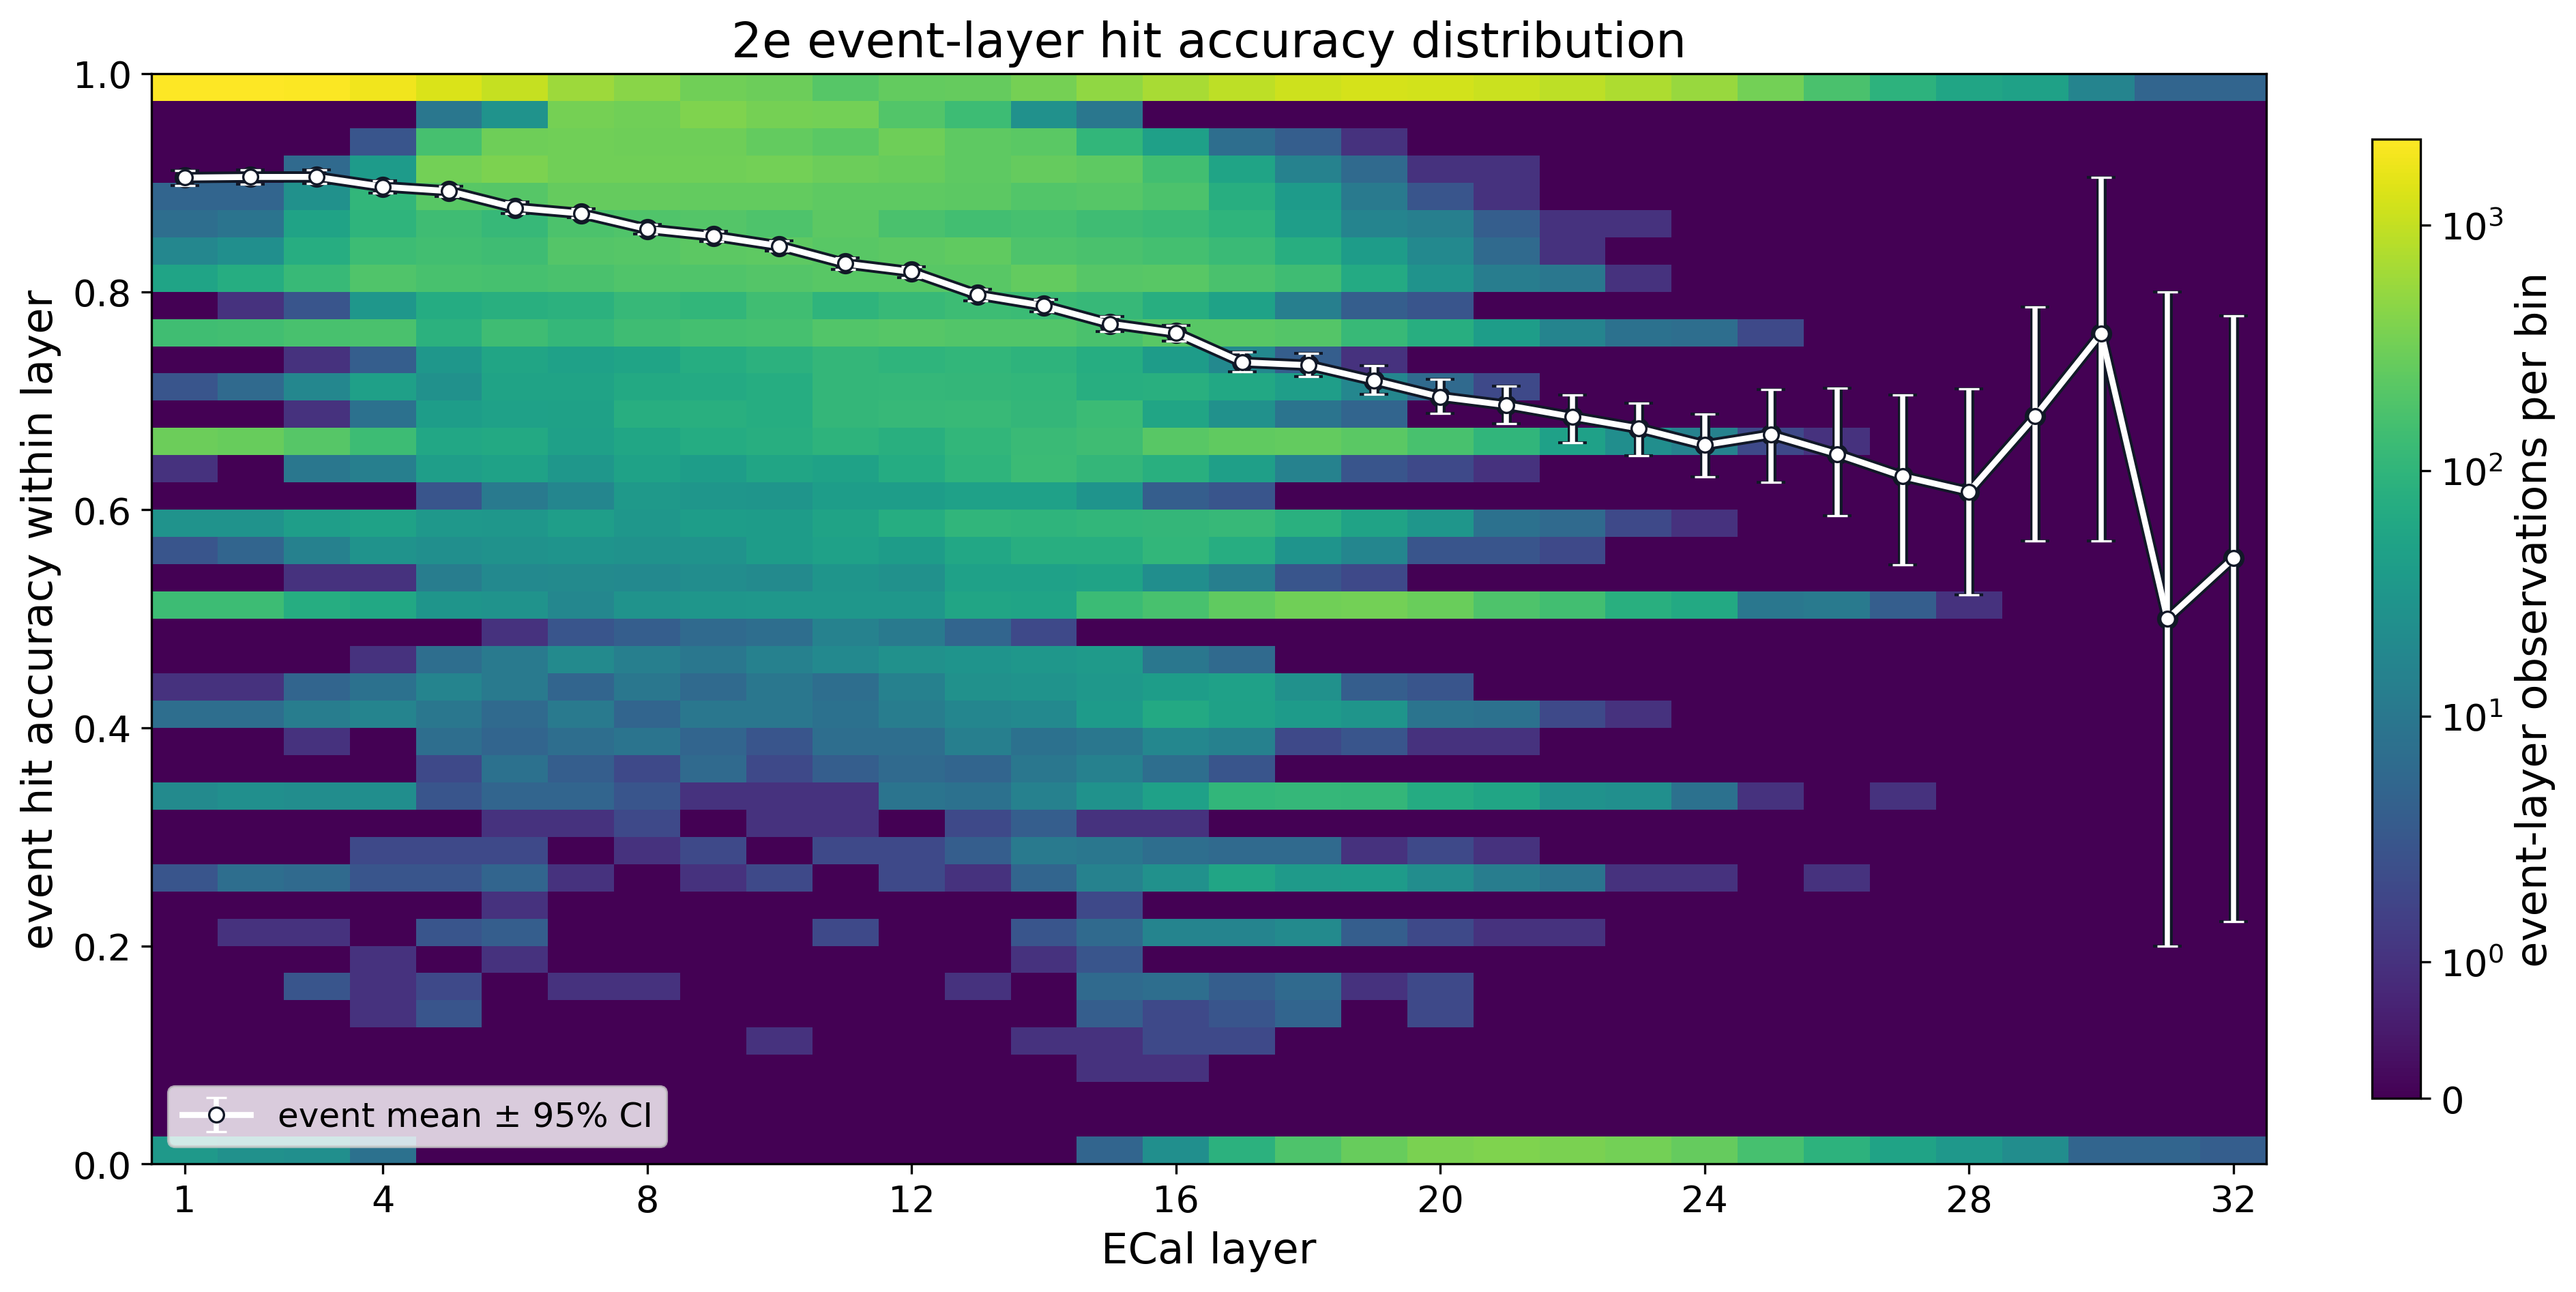
\includegraphics[width=0.98\linewidth]{config/fig/results/hit_accuracy_by_layer_2e.png}
    \vspace{0.5em}
    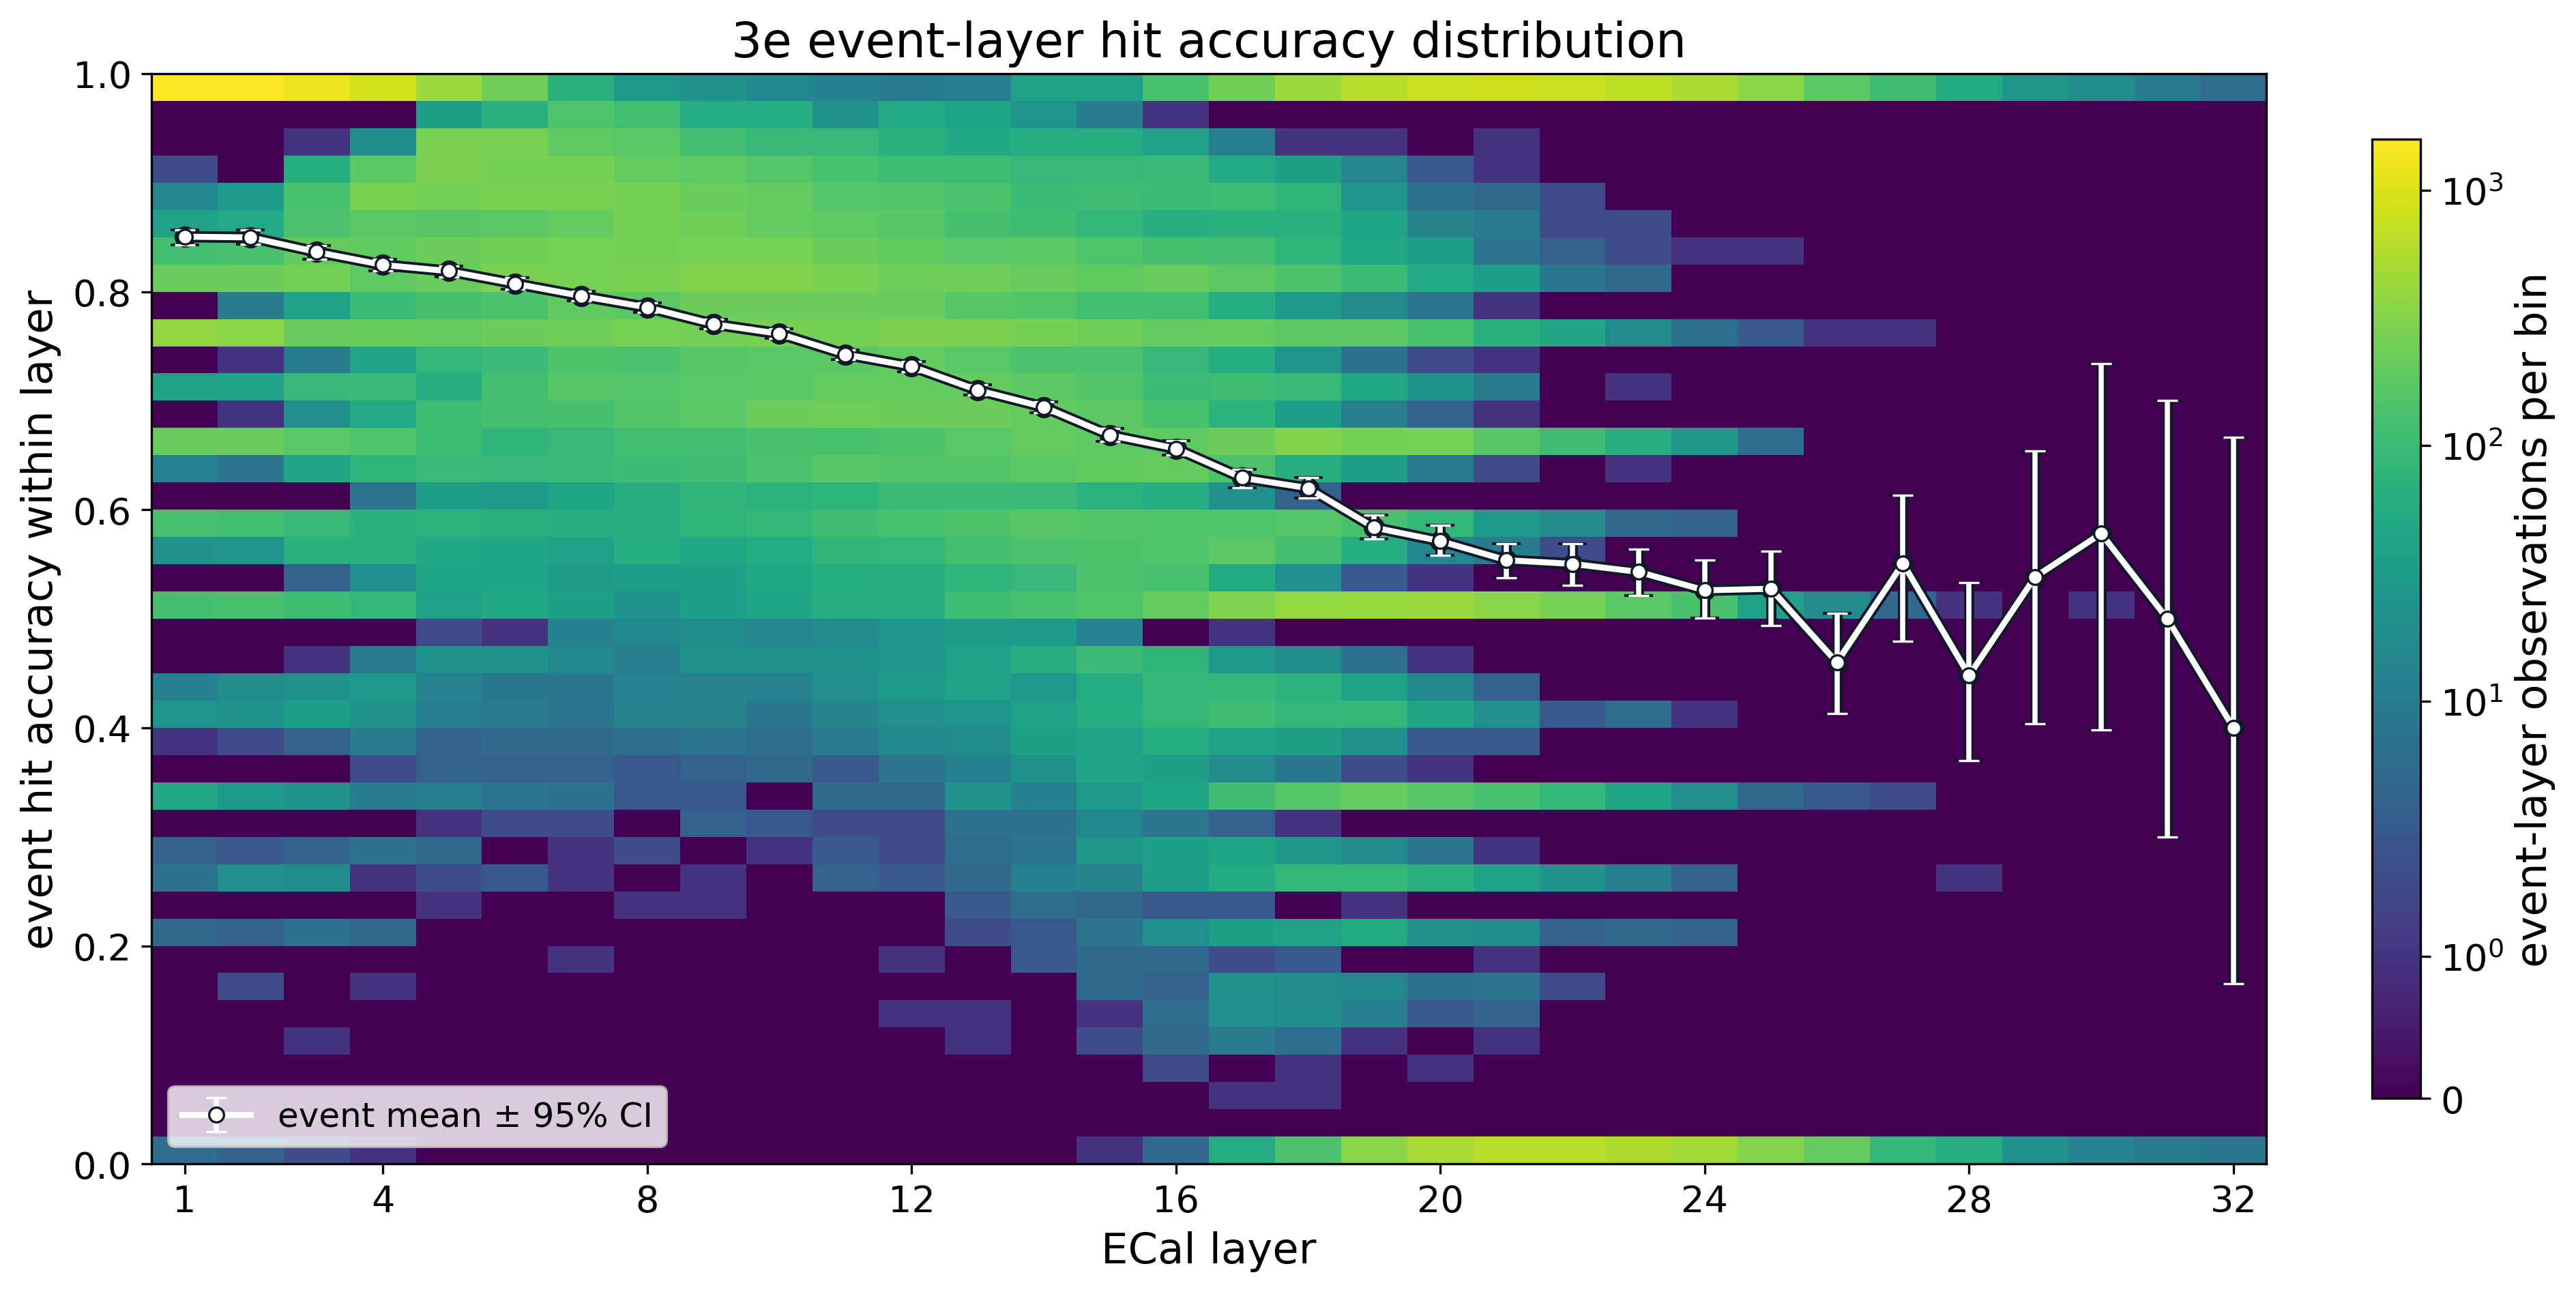
\includegraphics[width=0.98\linewidth]{config/fig/results/hit_accuracy_by_layer_3e.png}
    \caption{Distribution of permutation-aligned event-layer hit accuracy for
    \(2e\) events (top) and \(3e\) events (bottom). Color shows the number of
    event-layer observations in each rectangular bin on a logarithmic scale.
    White points show event-balanced means with \(95\,\%\) bootstrap confidence
    intervals.}
    \label{fig:results_layer_hit_accuracy}
\end{figure}

\begin{figure}[htbp]
    \centering
    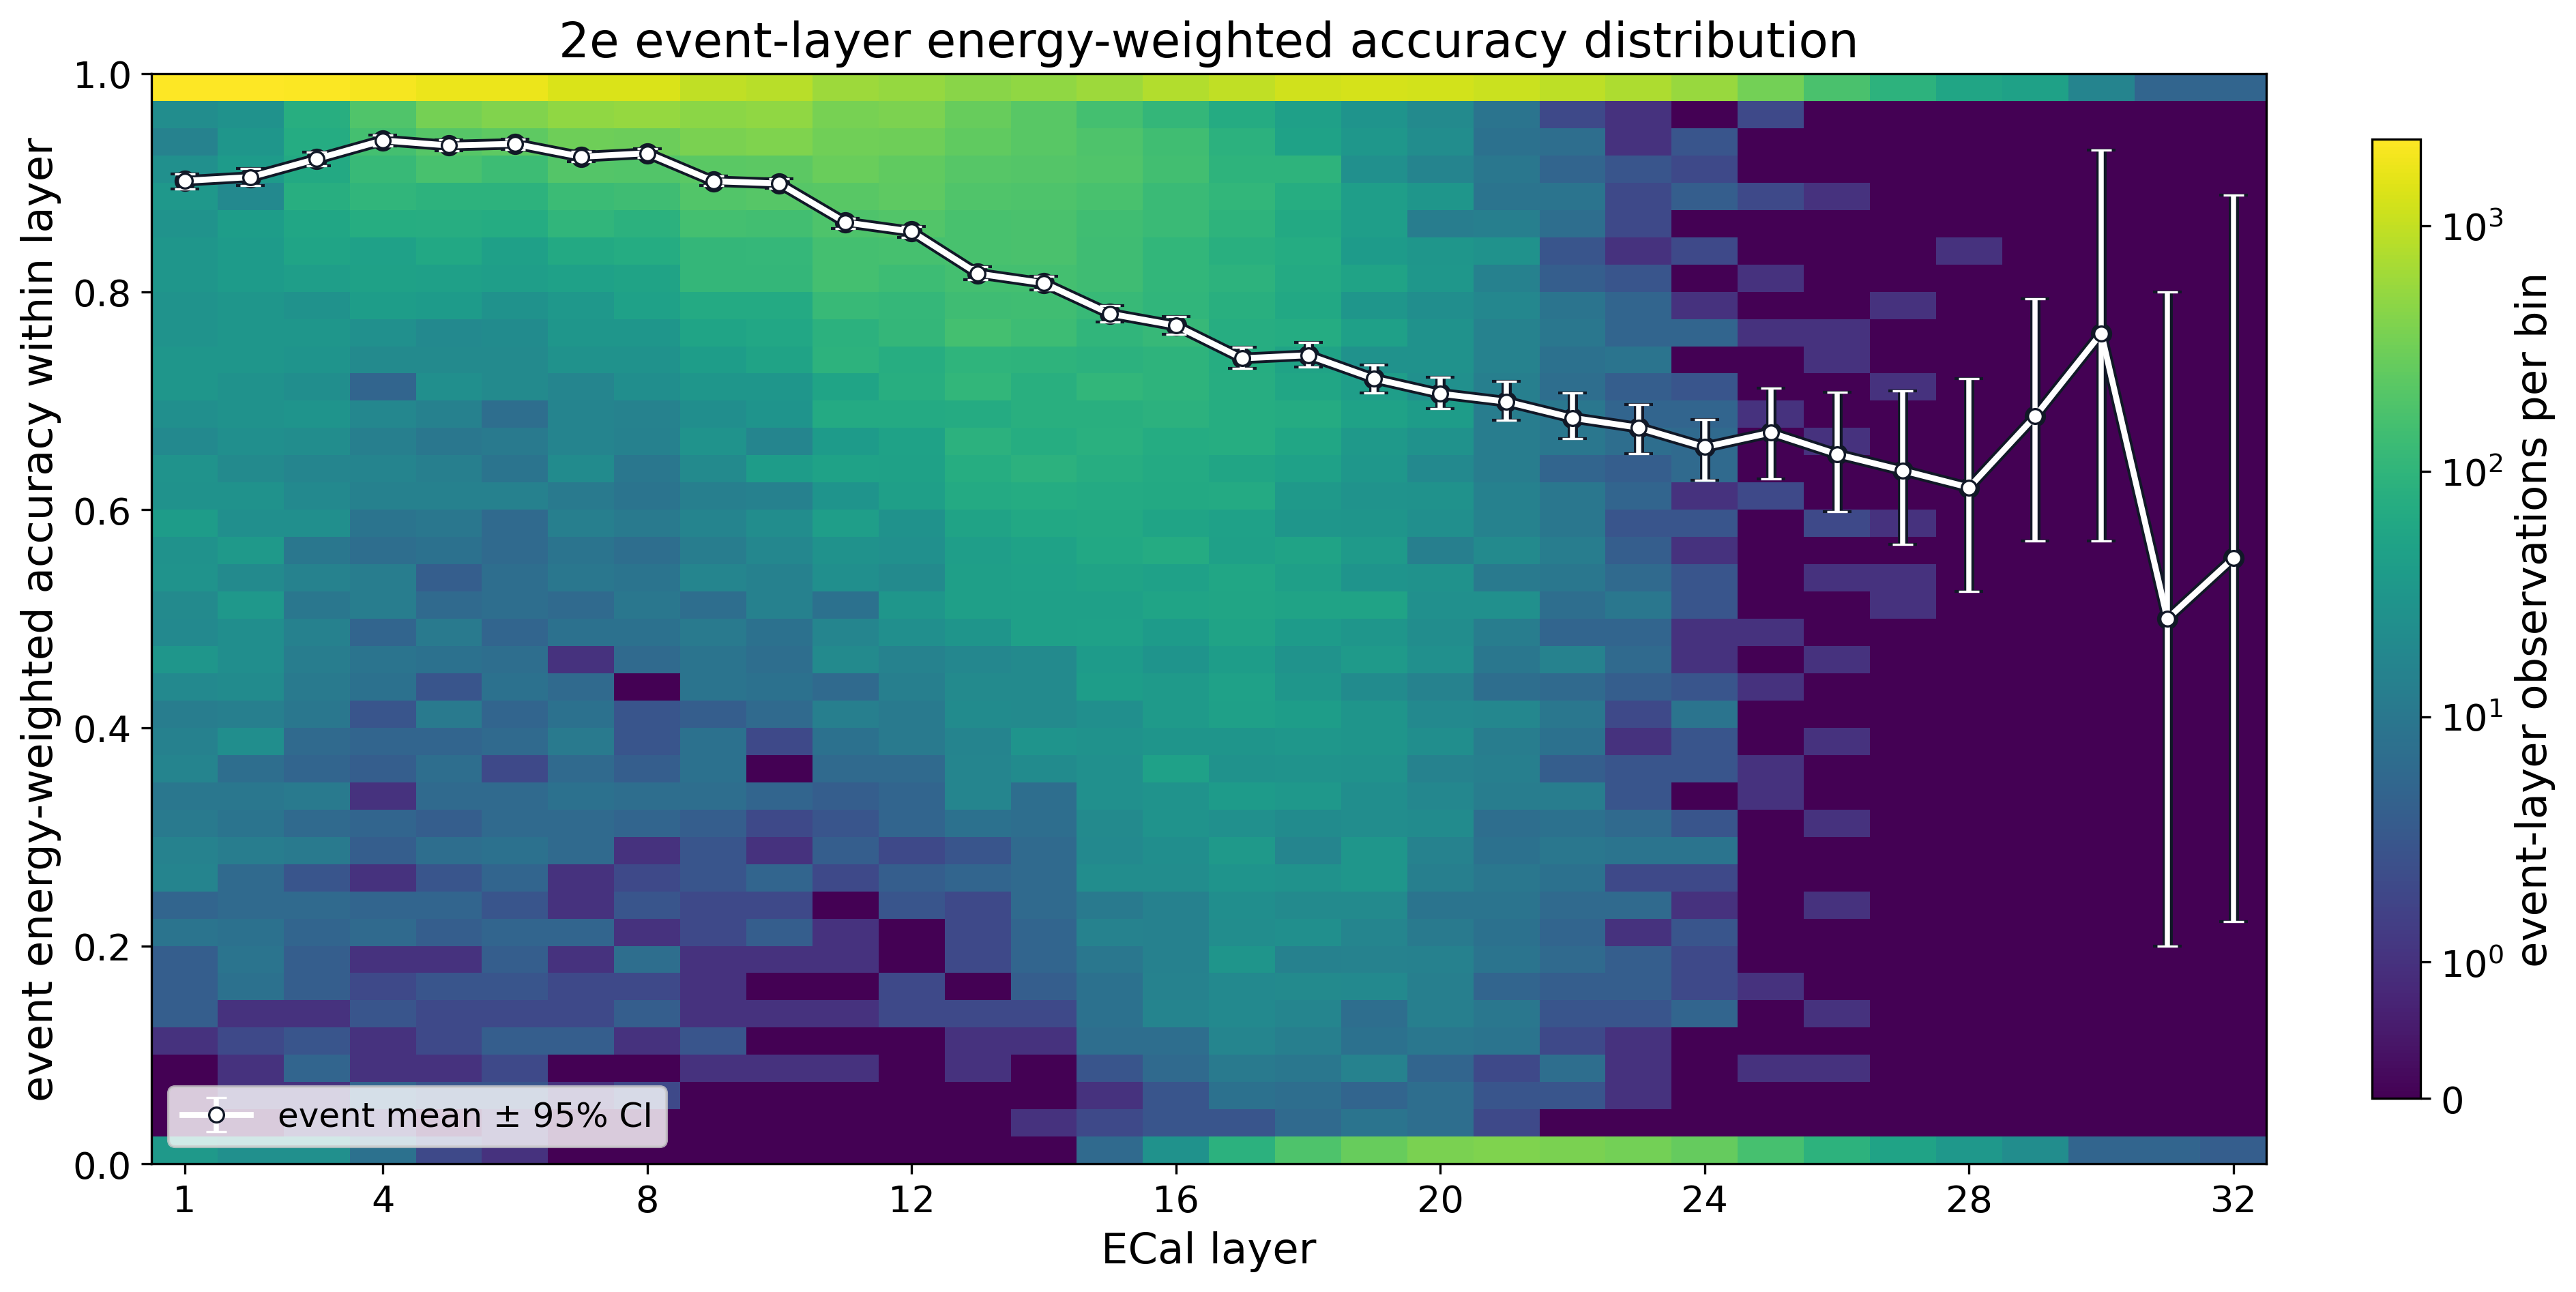
\includegraphics[width=0.98\linewidth]{config/fig/results/energy_weighted_accuracy_by_layer_2e.png}
    \vspace{0.5em}
    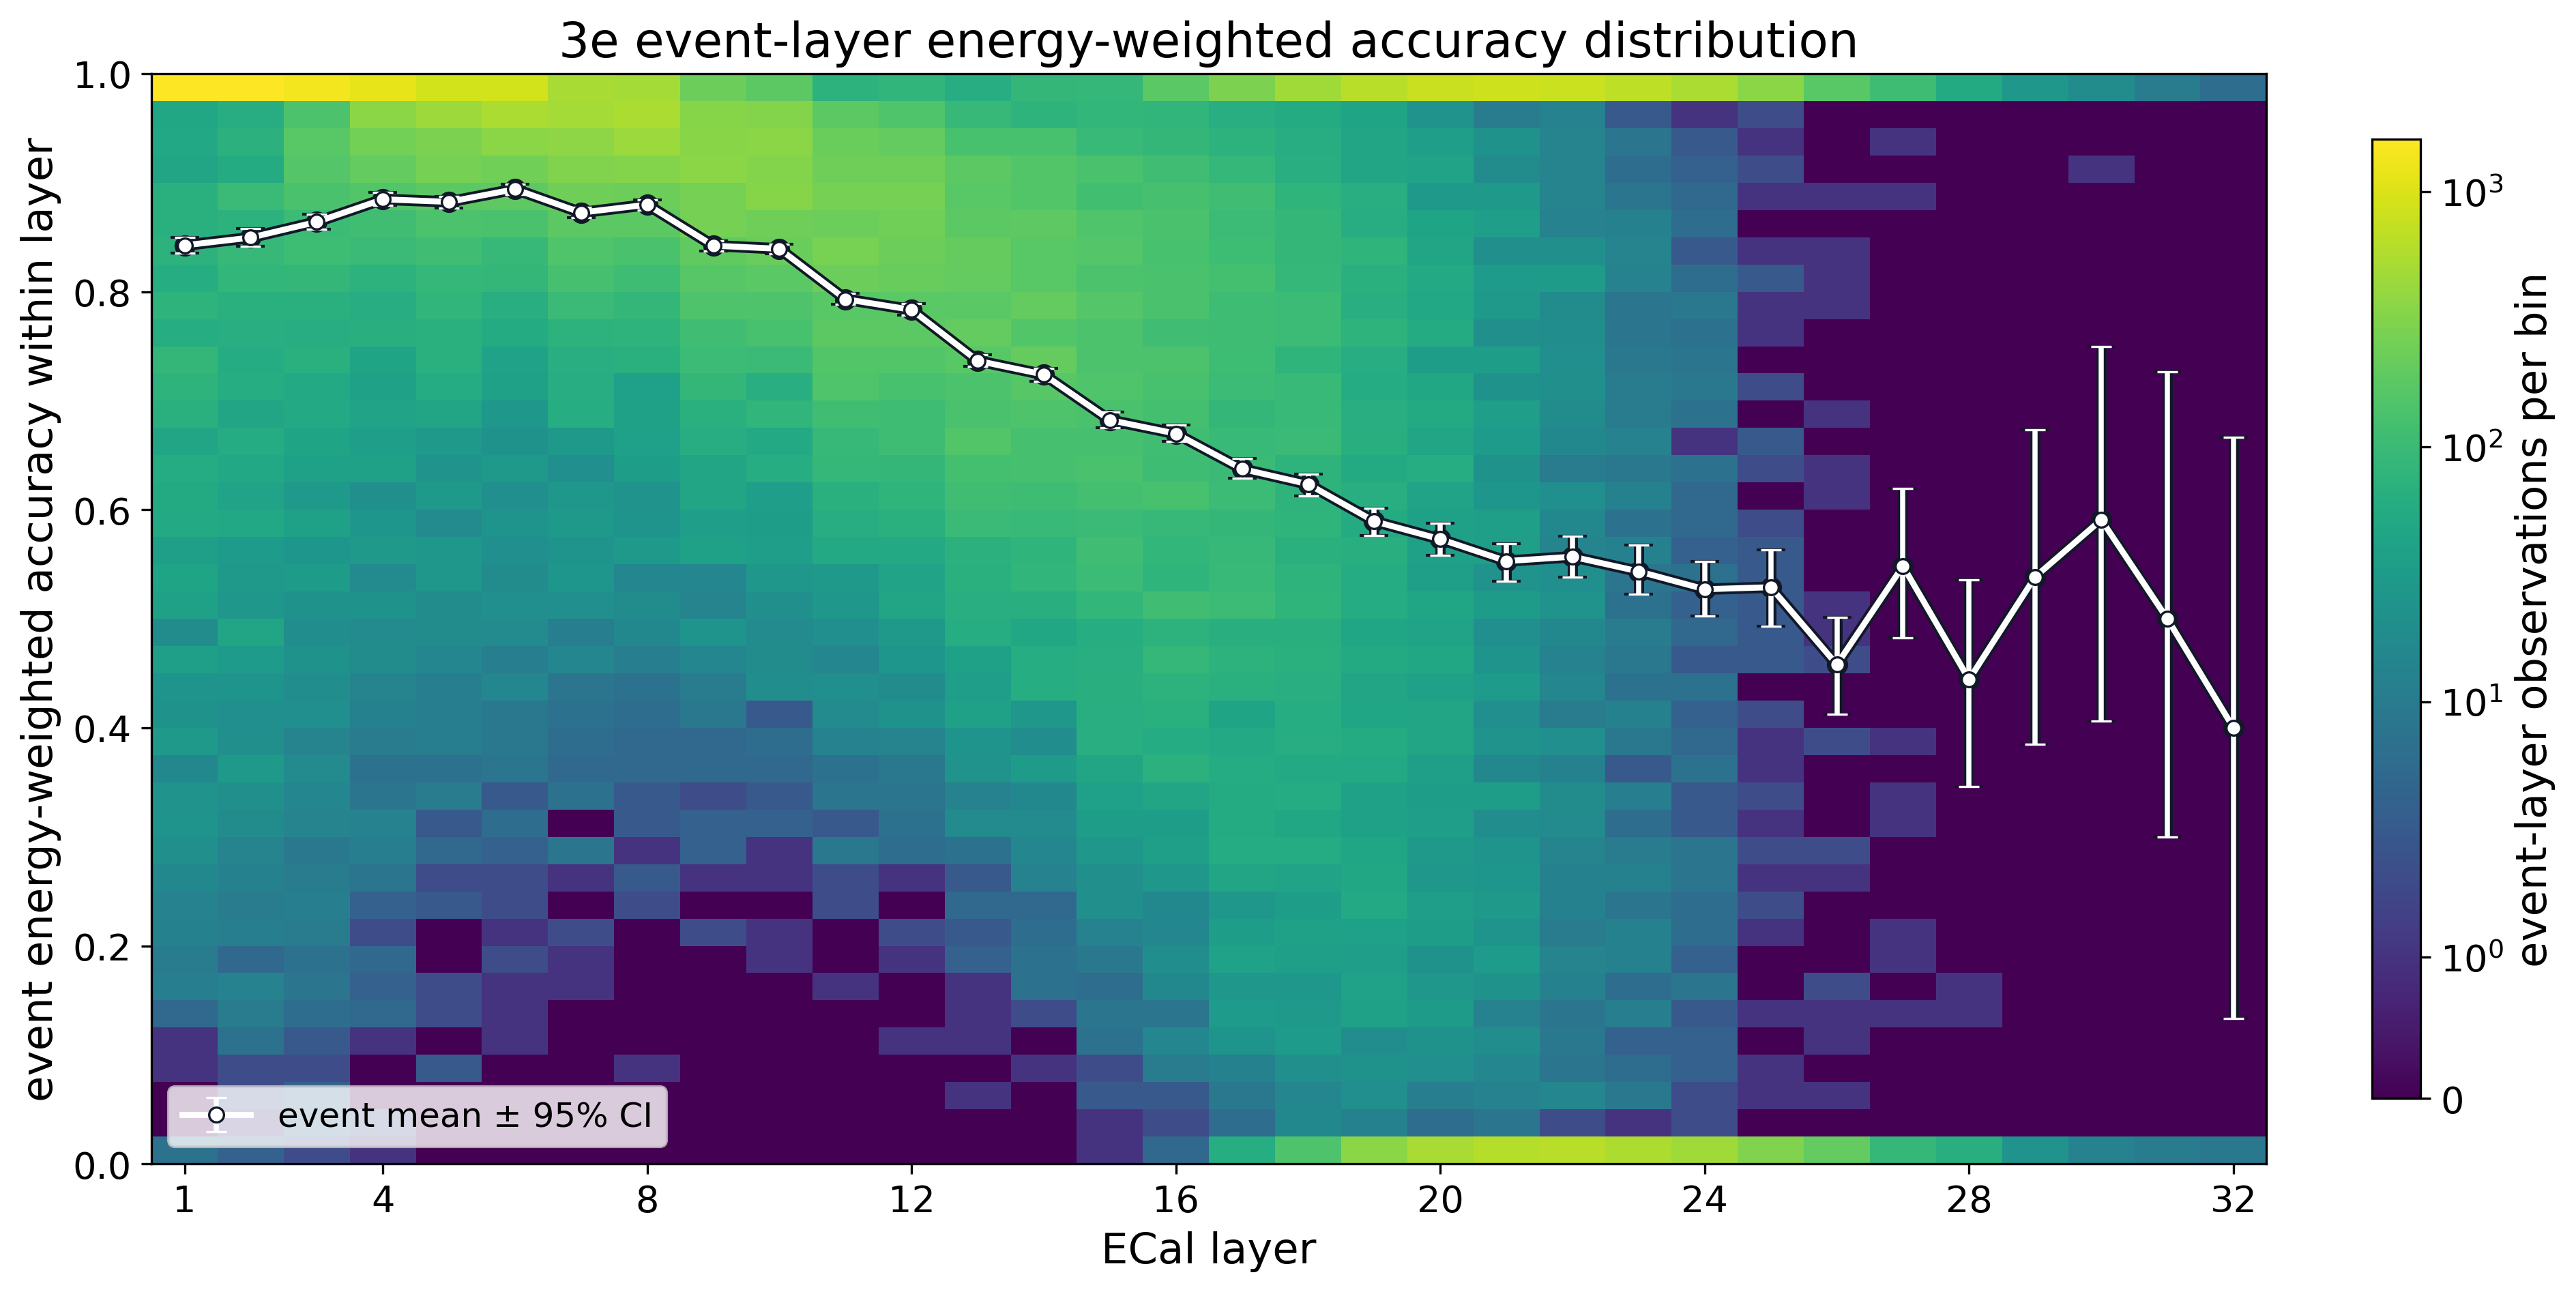
\includegraphics[width=0.98\linewidth]{config/fig/results/energy_weighted_accuracy_by_layer_3e.png}
    \caption{Distribution of raw-energy-weighted event-layer accuracy for
    \(2e\) events (top) and \(3e\) events (bottom), using the same event-wide
    label alignment as Figure~\ref{fig:results_layer_hit_accuracy}. White
    points show event-balanced means with \(95\,\%\) bootstrap confidence
    intervals.}
    \label{fig:results_layer_energy_accuracy}
\end{figure}

Over all layers, the energy-weighted accuracies are \(0.888\) for \(2e\) and
\(0.825\) for \(3e\), both higher than their corresponding unweighted hit
accuracies. Within this development sample, incorrectly assigned hits
therefore carry less reconstructed energy on average than correctly assigned
hits. The depth dependence nevertheless remains, showing that energy weighting
does not remove the loss of separation quality in the later shower region.

\clearpage
\subsection{Dependence on Shower Separation}

The following plots relate event accuracy to truth-assisted geometric
descriptions of shower overlap. For these development diagnostics, the weight
of hit \(h\) in the geometry of origin \(j\) is the product of its raw
reconstructed energy and the simulated deposited-energy fraction from that
origin. These fractions are simulation truth, so the resulting quantities are
oracle difficulty diagnostics rather than observables available in measured
detector data. Figure~\ref{fig:results_moliere_separation} uses the smallest pairwise
distance between these energy-weighted shower centroids. Dividing by the
reference Moli\`ere radius \(R_{\mathrm{M}}=25\,\mathrm{mm}\) supplies an
interpretable detector scale, but the line at one Moli\`ere radius is not a hard
resolution boundary.

\begin{figure}[htbp]
    \centering
    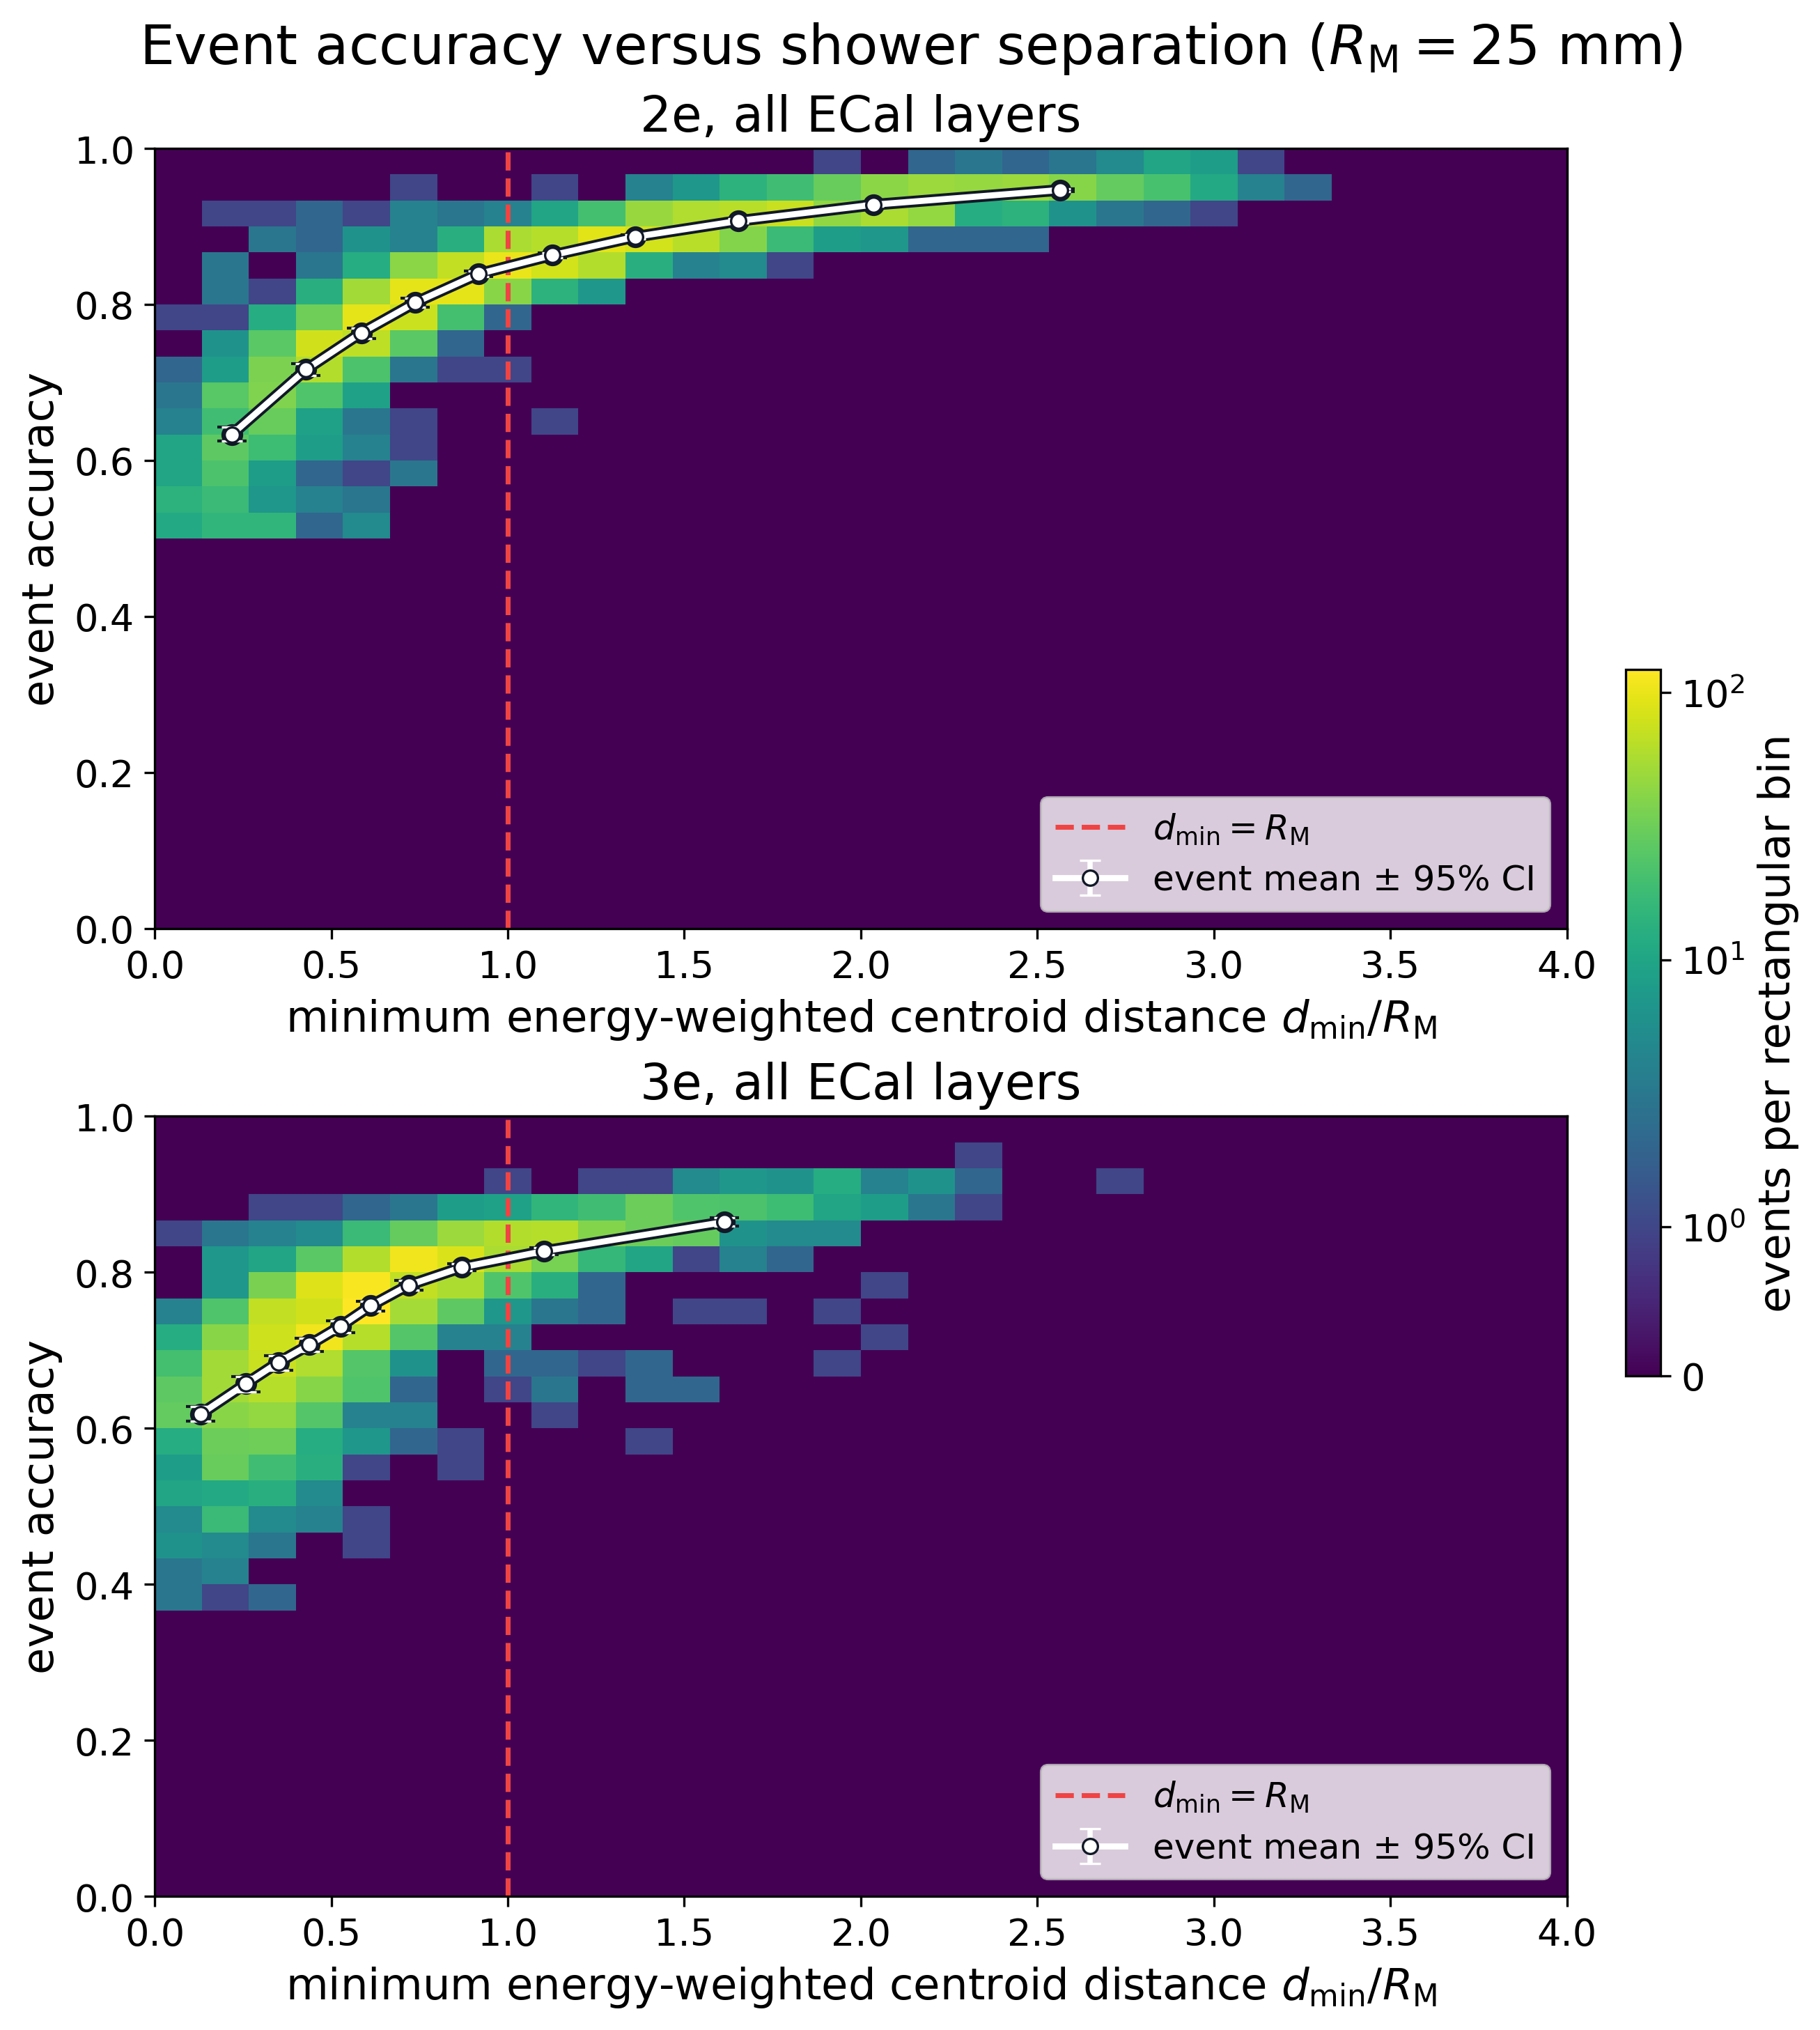
\includegraphics[height=0.72\textheight,keepaspectratio]{config/fig/results/separation_in_moliere_units.png}
    \caption{Permutation-aligned event hit accuracy as a function of the
    minimum energy-weighted centroid separation in units of
    \(R_{\mathrm{M}}=25\,\mathrm{mm}\), for \(2e\) events (top) and \(3e\)
    events (bottom). White points show equal-population bin means with
    \(95\,\%\) bootstrap confidence intervals. The red line marks one Moli\`ere
    radius as an interpretive scale.}
    \label{fig:results_moliere_separation}
\end{figure}

The event mean rises as the minimum centroid distance increases. The trend is
present for both multiplicities and is consistent with shower overlap being a
major source of assignment ambiguity. The sizeable accuracy spread at a fixed
distance also shows that centroid separation is not a complete description of
event difficulty.

Figure~\ref{fig:results_width_separation} instead divides the minimum centroid
distance by the combined energy-weighted root-mean-square widths of the two
showers. This produces a dimensionless overlap measure and separates the
all-layer geometry from the geometry in the first three layers.

\begin{figure}[htbp]
    \centering
    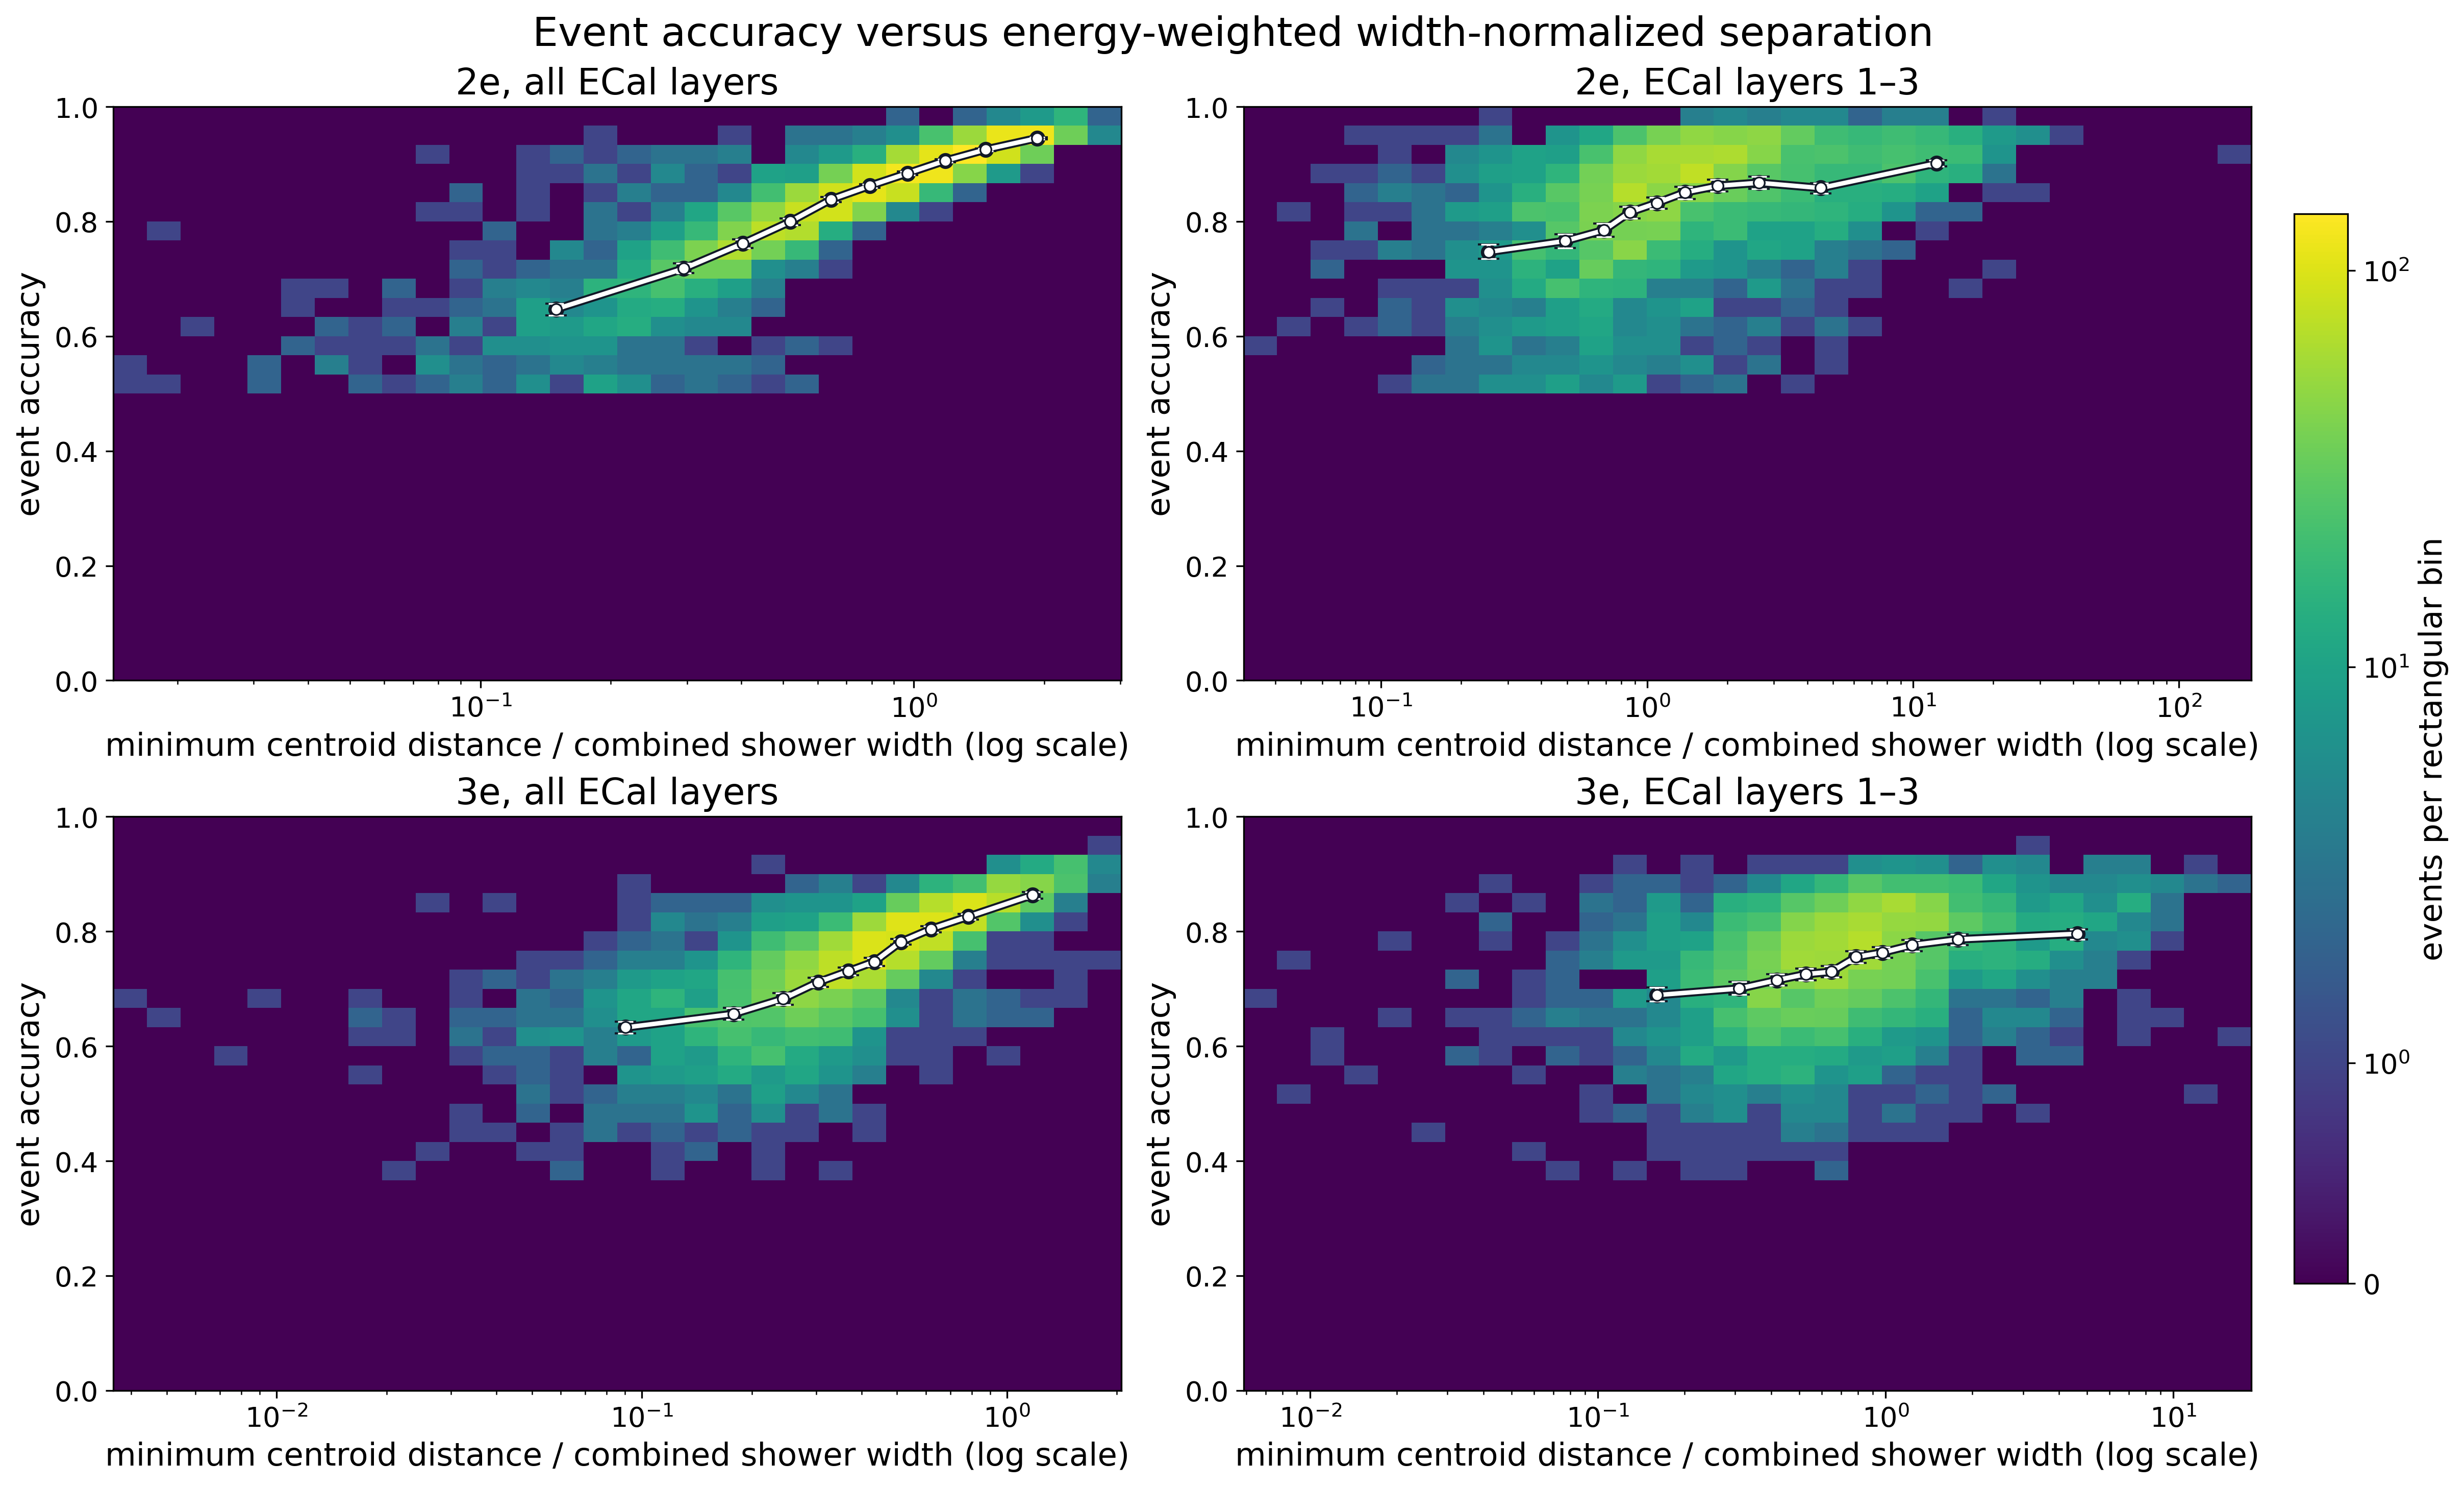
\includegraphics[width=0.99\linewidth]{config/fig/results/width_normalized_separation.png}
    \caption{Permutation-aligned event hit accuracy as a function of minimum
    energy-weighted centroid distance divided by combined shower width. The
    left column uses all ECal layers and the right column uses layers 1--3;
    \(2e\) events are shown above \(3e\) events. The horizontal axes are
    logarithmic.}
    \label{fig:results_width_separation}
\end{figure}

The all-layer profiles again show increasing accuracy with separation. The
first-three-layer profiles retain a weaker trend, indicating that the initial
shower geometry contains useful information but does not fully determine the
separability of the developed shower.

\clearpage
\subsection{Confidence and Selective Performance}

The negative relation between prediction entropy and event accuracy in
Figure~\ref{fig:results_entropy} shows that the model is generally less
certain on events that it reconstructs poorly. Mean normalised entropy can
therefore help rank difficult events, although this correlation does not make
it a complete or independently calibrated measure of reconstruction quality.

\begin{figure}[htbp]
    \centering
    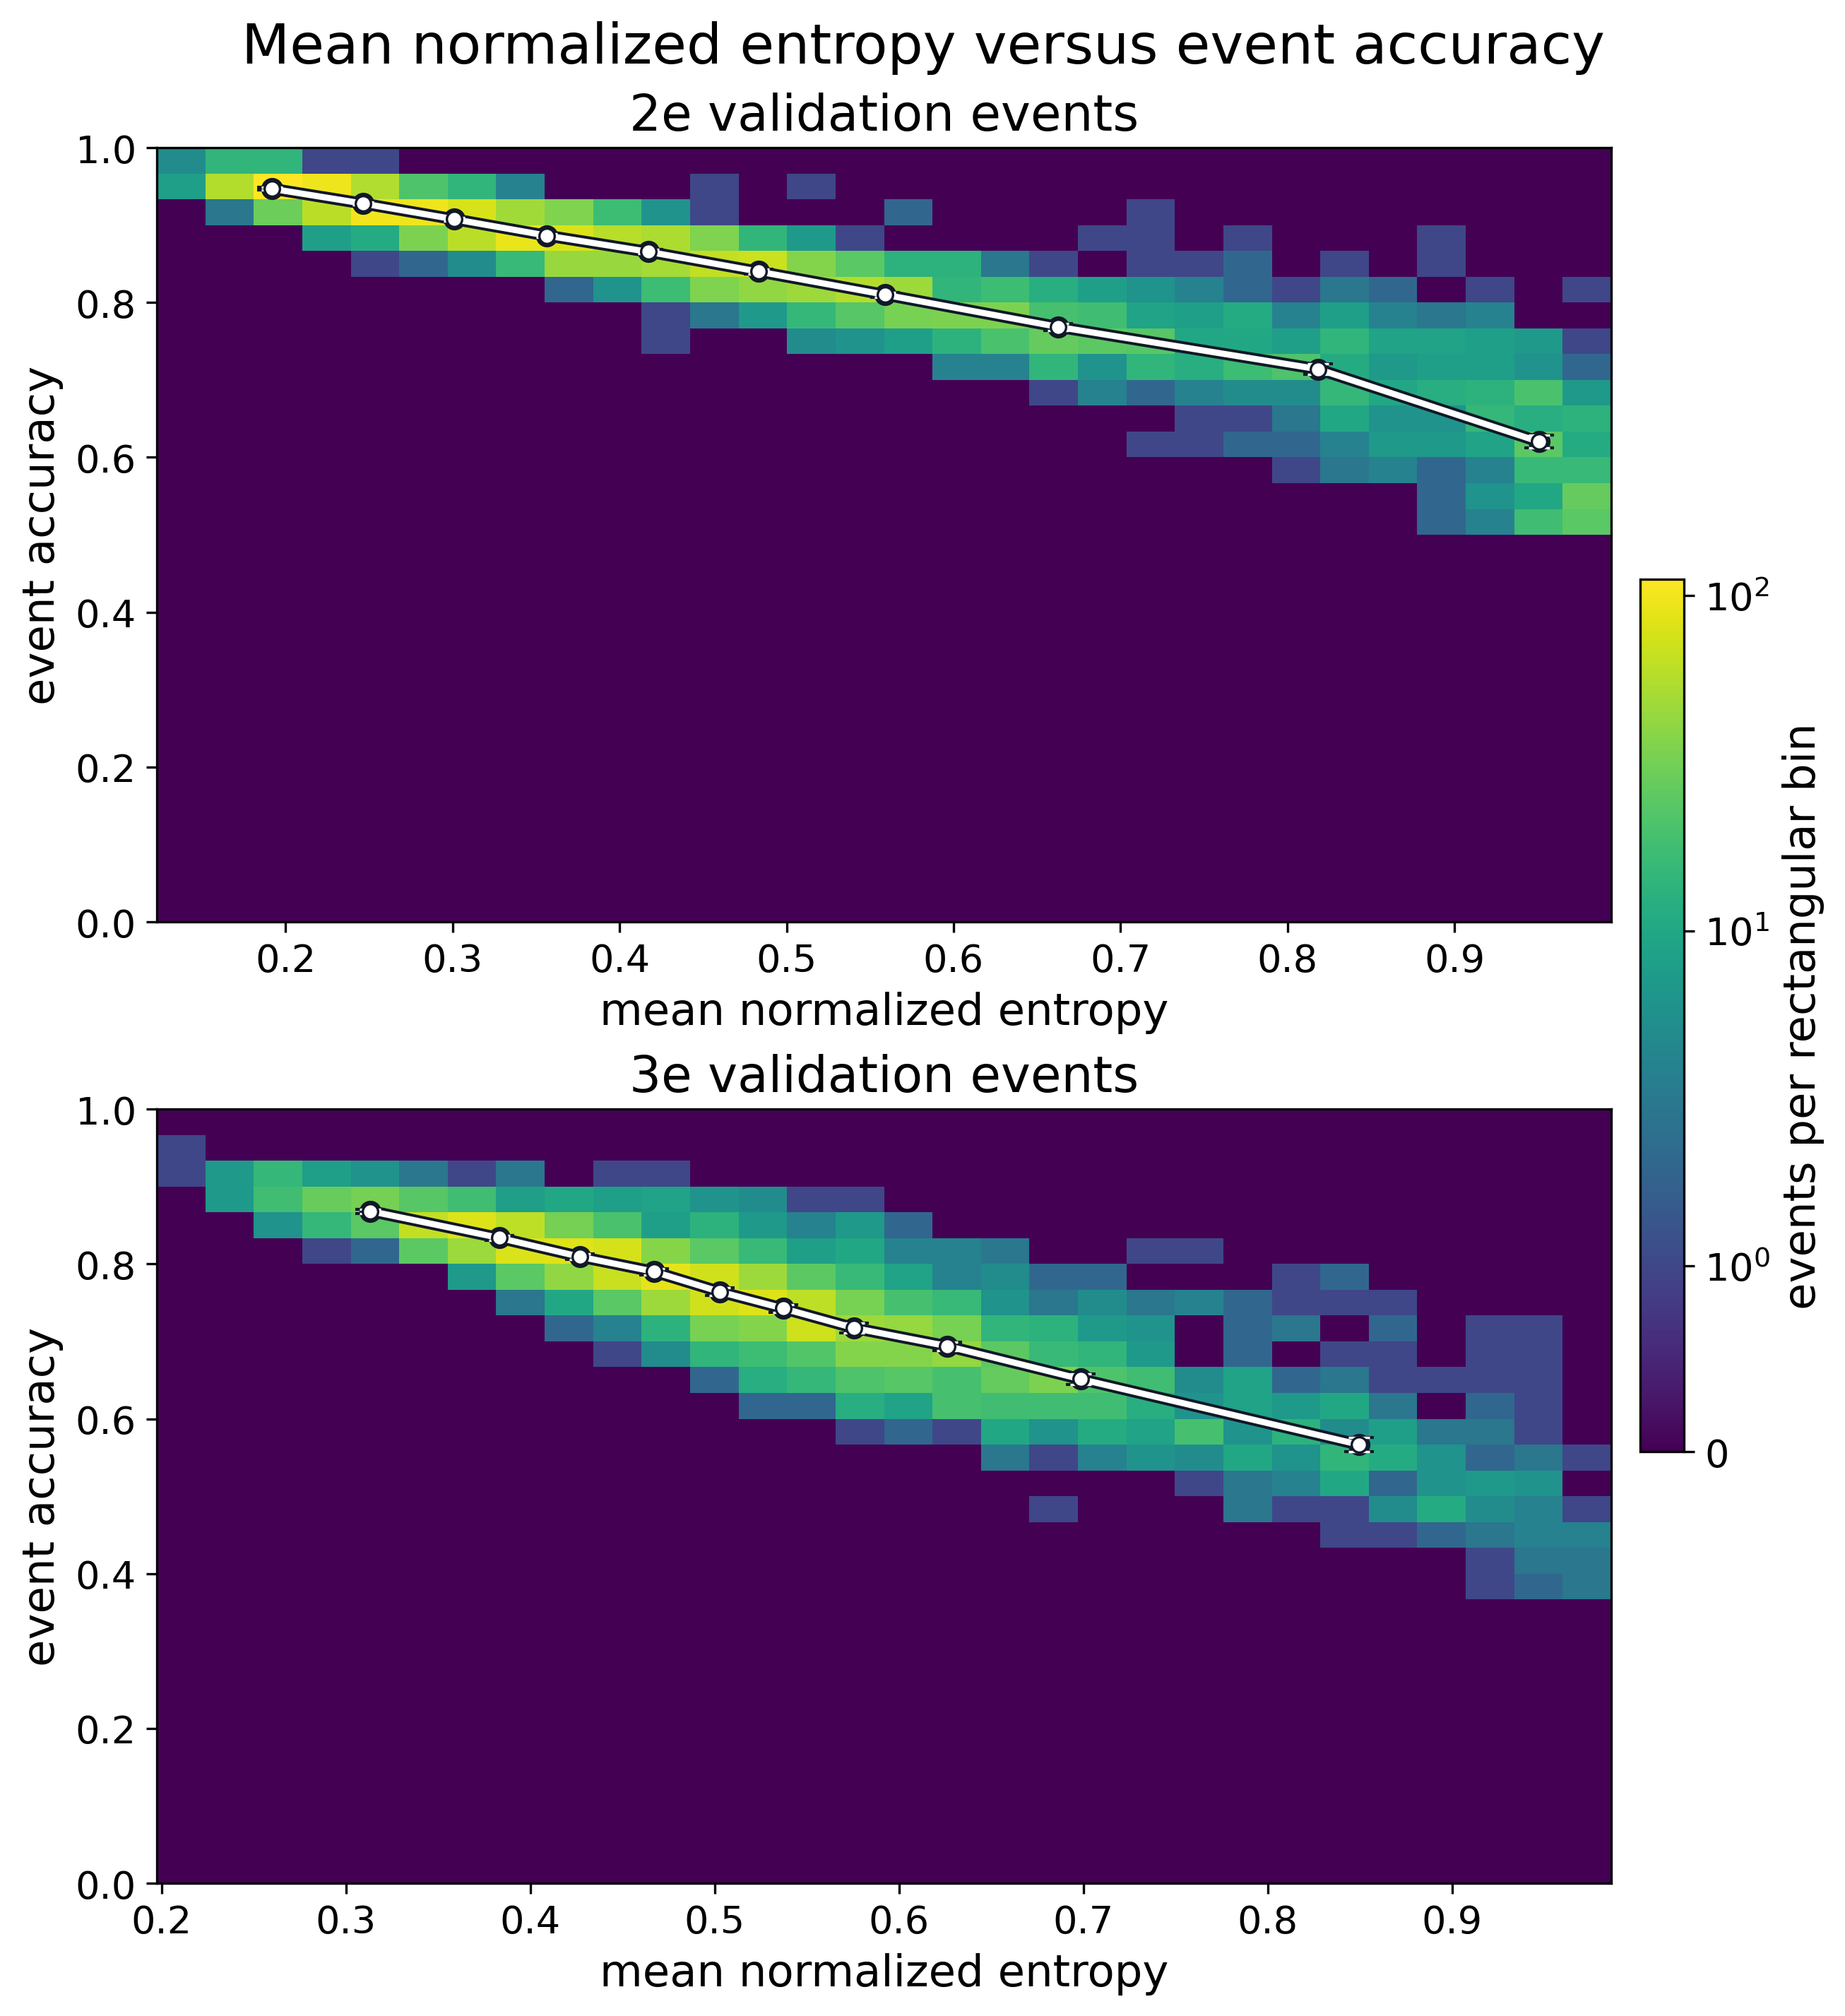
\includegraphics[width=0.96\linewidth,height=0.72\textheight,keepaspectratio]{config/fig/results/entropy_vs_event_accuracy.png}
    \caption{Mean normalized prediction entropy against permutation-aligned
    event hit accuracy for \(2e\) events (top) and \(3e\) events (bottom).
    White points show equal-population bin means with \(95\,\%\) bootstrap
    confidence intervals.}
    \label{fig:results_entropy}
\end{figure}

Figure~\ref{fig:results_accuracy_coverage} makes the corresponding selection
trade-off explicit. Retaining only high-confidence hits increases their
accuracy, but reduces hit coverage. The retained energy fraction decreases
more slowly than the retained hit fraction, indicating that many of the first
hits removed carry relatively little reconstructed energy. Selecting complete
events by confidence gives a smaller but consistent increase in mean event
accuracy as coverage is reduced.

\begin{figure}[htbp]
    \centering
    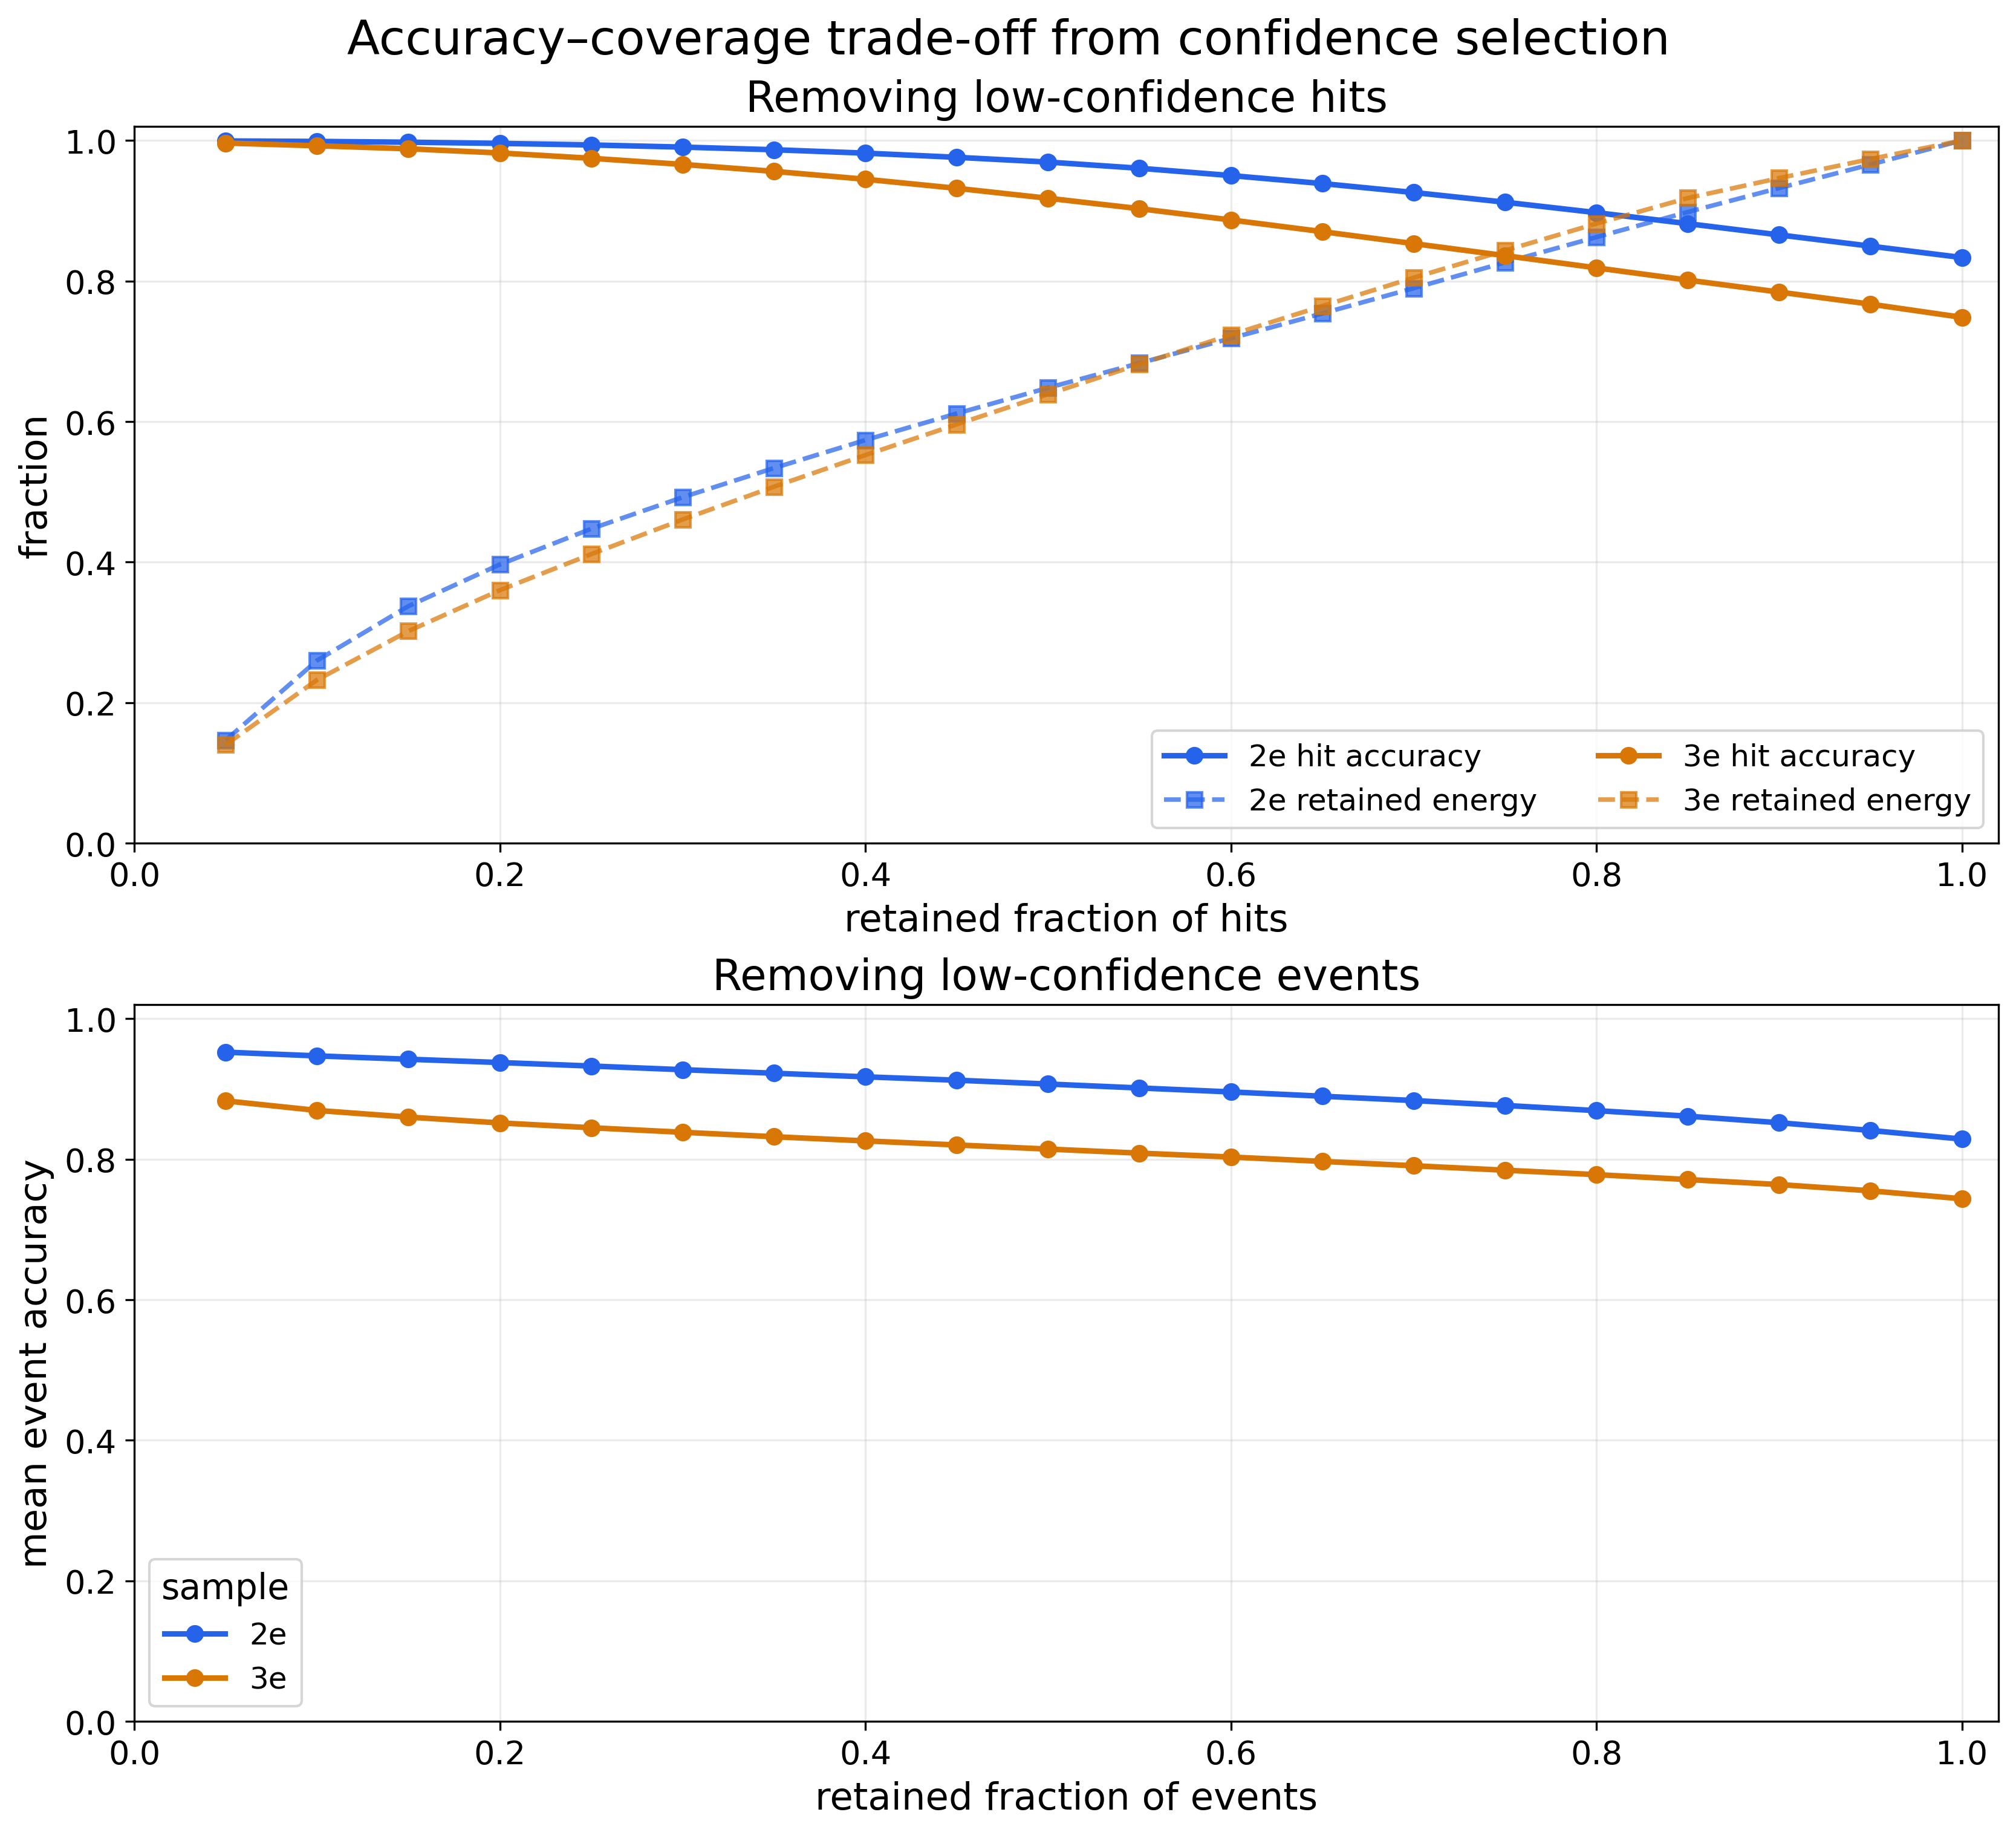
\includegraphics[width=0.94\linewidth]{config/fig/results/accuracy_coverage.png}
    \caption{Accuracy-coverage trade-off obtained by ordering predictions by
    confidence. The upper panel removes low-confidence hits and shows both the
    accuracy and retained raw-energy fraction. The lower panel removes
    complete low-confidence events and shows the mean accuracy of the retained
    events.}
    \label{fig:results_accuracy_coverage}
\end{figure}

The layer profiles in Figure~\ref{fig:results_layer_confidence} show that mean
confidence and mean accuracy follow each other closely through most of the
ECal. Their separation and uncertainty grow in the sparsely populated final
layers, where the per-layer estimate is least stable. Agreement between the
two layer means does not by itself establish hit-level probability
calibration.

\begin{figure}[htbp]
    \centering
    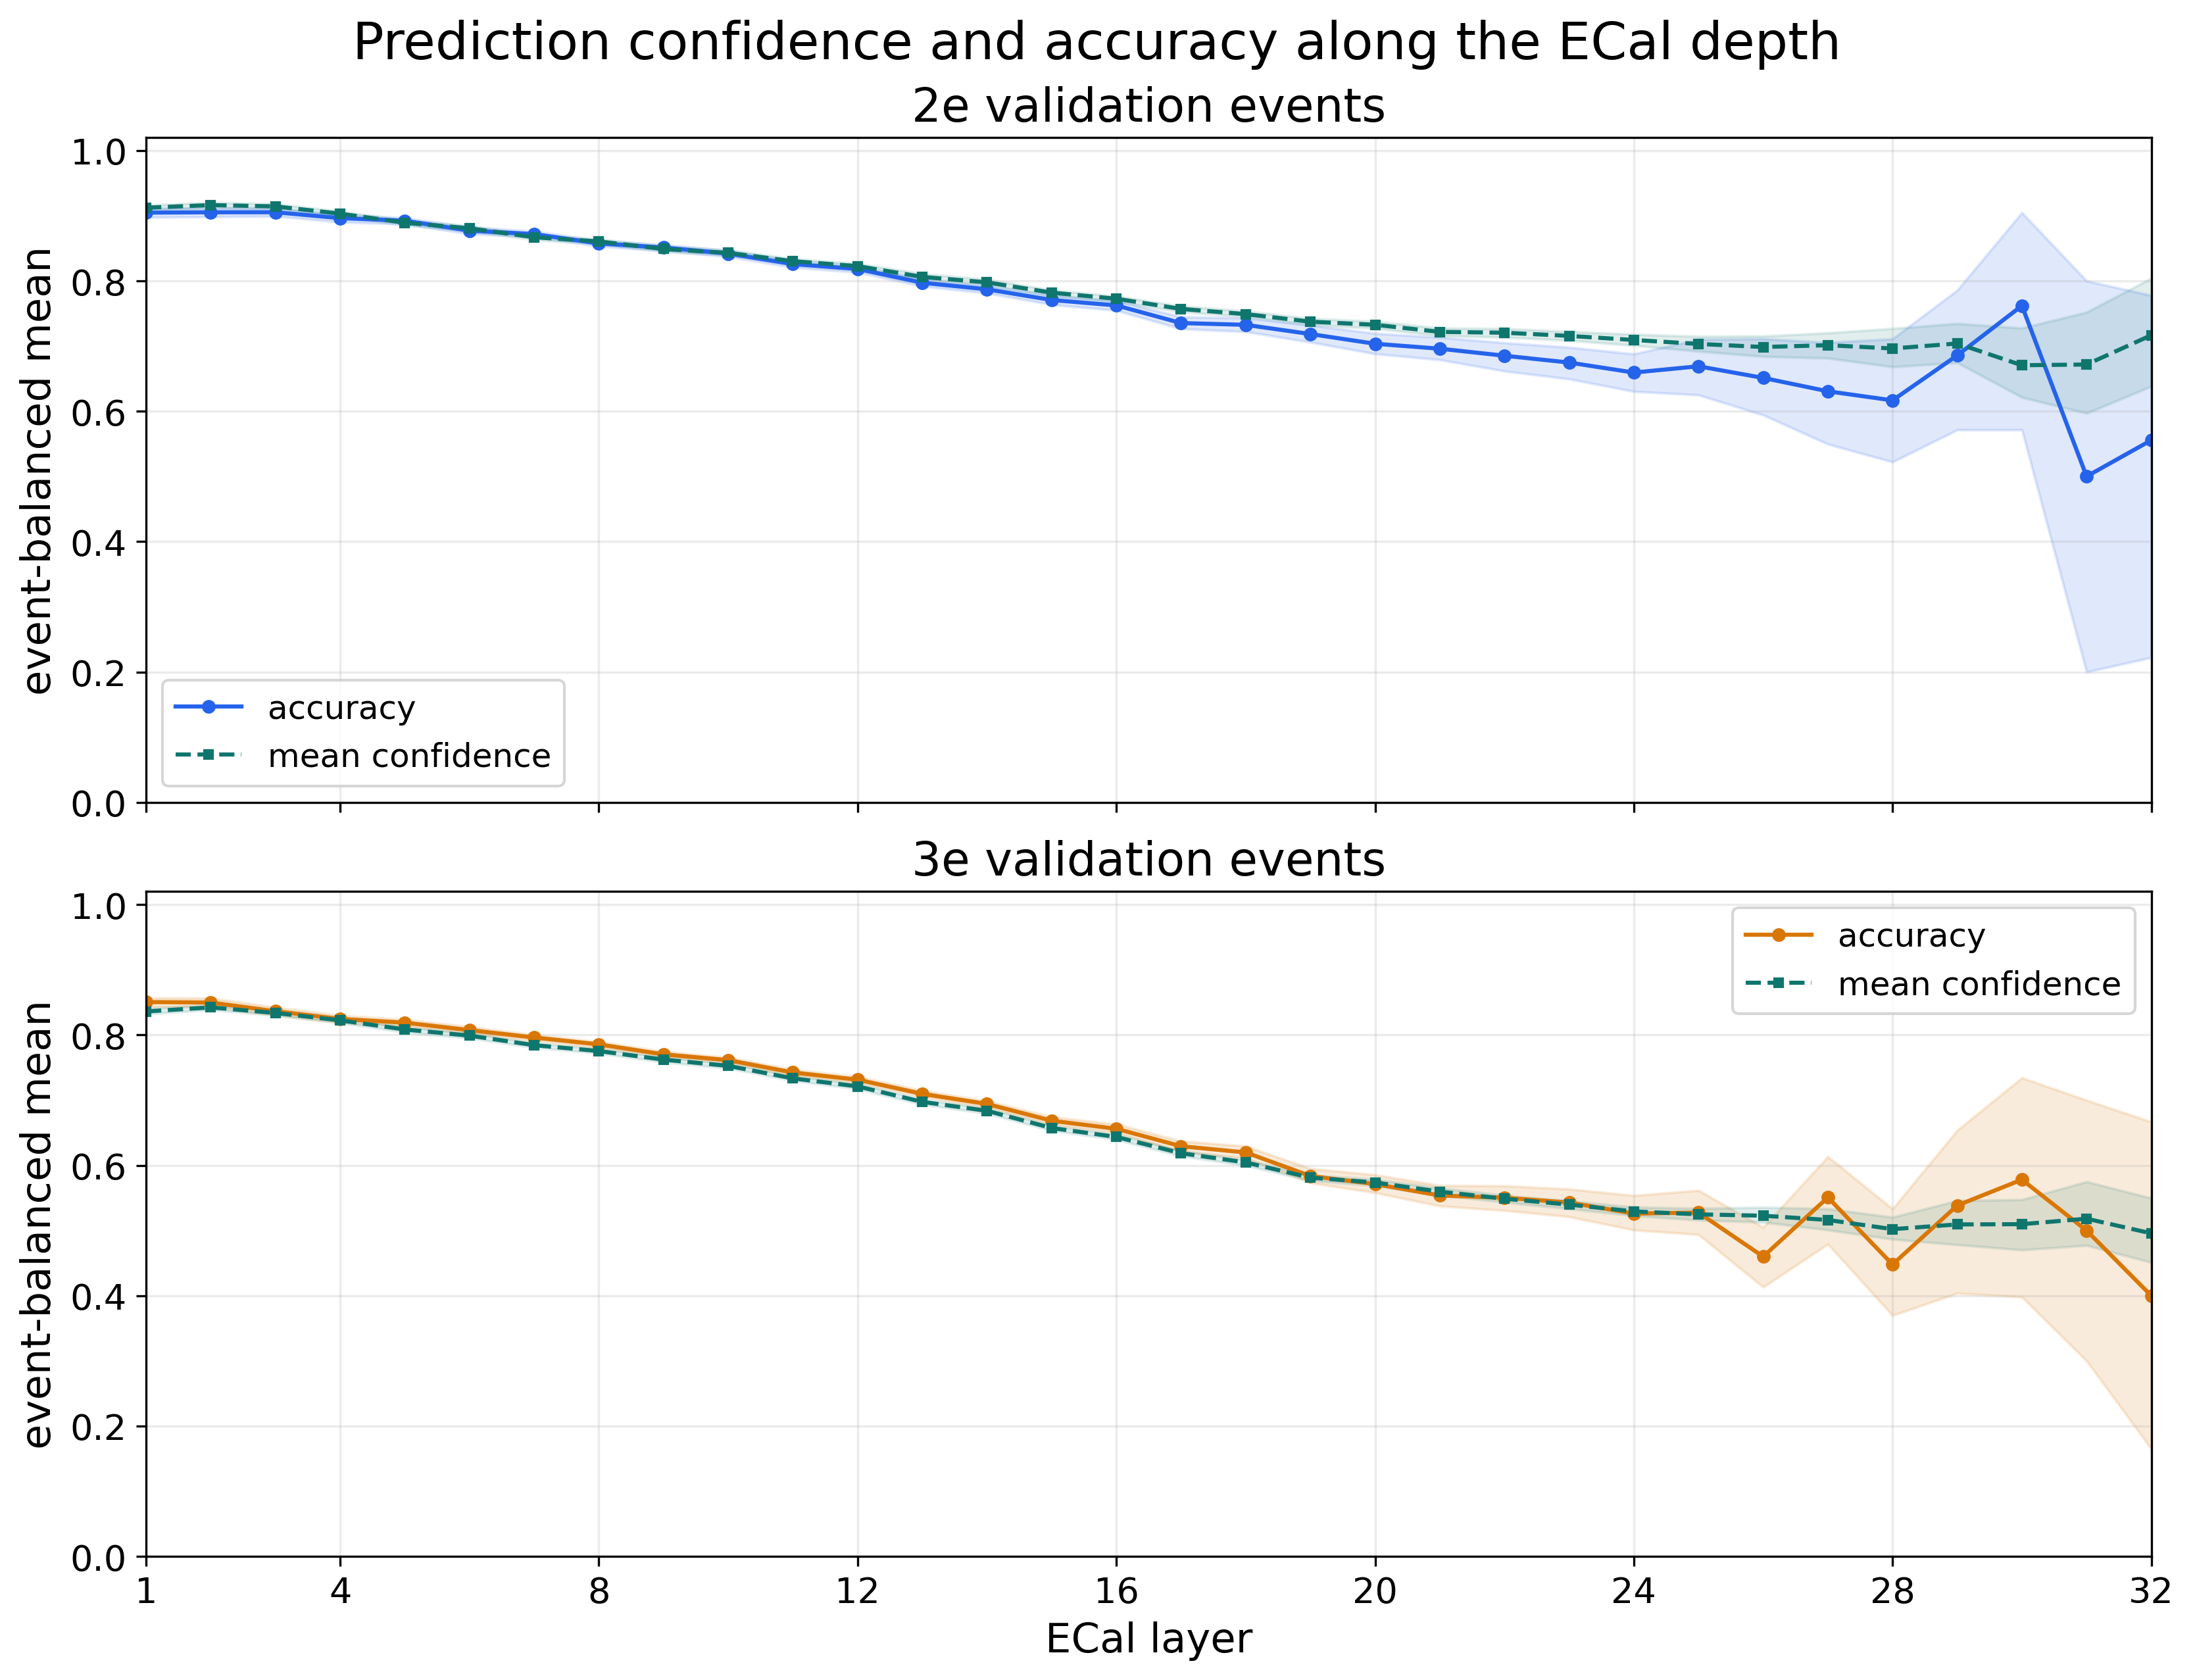
\includegraphics[width=0.96\linewidth]{config/fig/results/confidence_accuracy_by_layer.png}
    \caption{Event-balanced mean prediction confidence and
    permutation-aligned accuracy across the ECal depth for \(2e\) events
    (top) and \(3e\) events (bottom). Shaded bands show \(95\,\%\) bootstrap
    confidence intervals.}
    \label{fig:results_layer_confidence}
\end{figure}

\clearpage
\subsection{Trigger-Pad Ablation}

Figure~\ref{fig:results_tpad_ablation} removes trigger-pad-track tokens at
inference time from one trained \(3e\) \texttt{ECalTpadTransformer}. The
reference and ablated event accuracies are almost identical. Across the
\(3{,}000\) validation events, the pooled hit-accuracy gain from retaining the
trigger-pad inputs is \(1.26\times10^{-4}\), the mean event-accuracy gain is
\(1.32\times10^{-4}\), and the median event-accuracy gain is zero.

\begin{figure}[htbp]
    \centering
    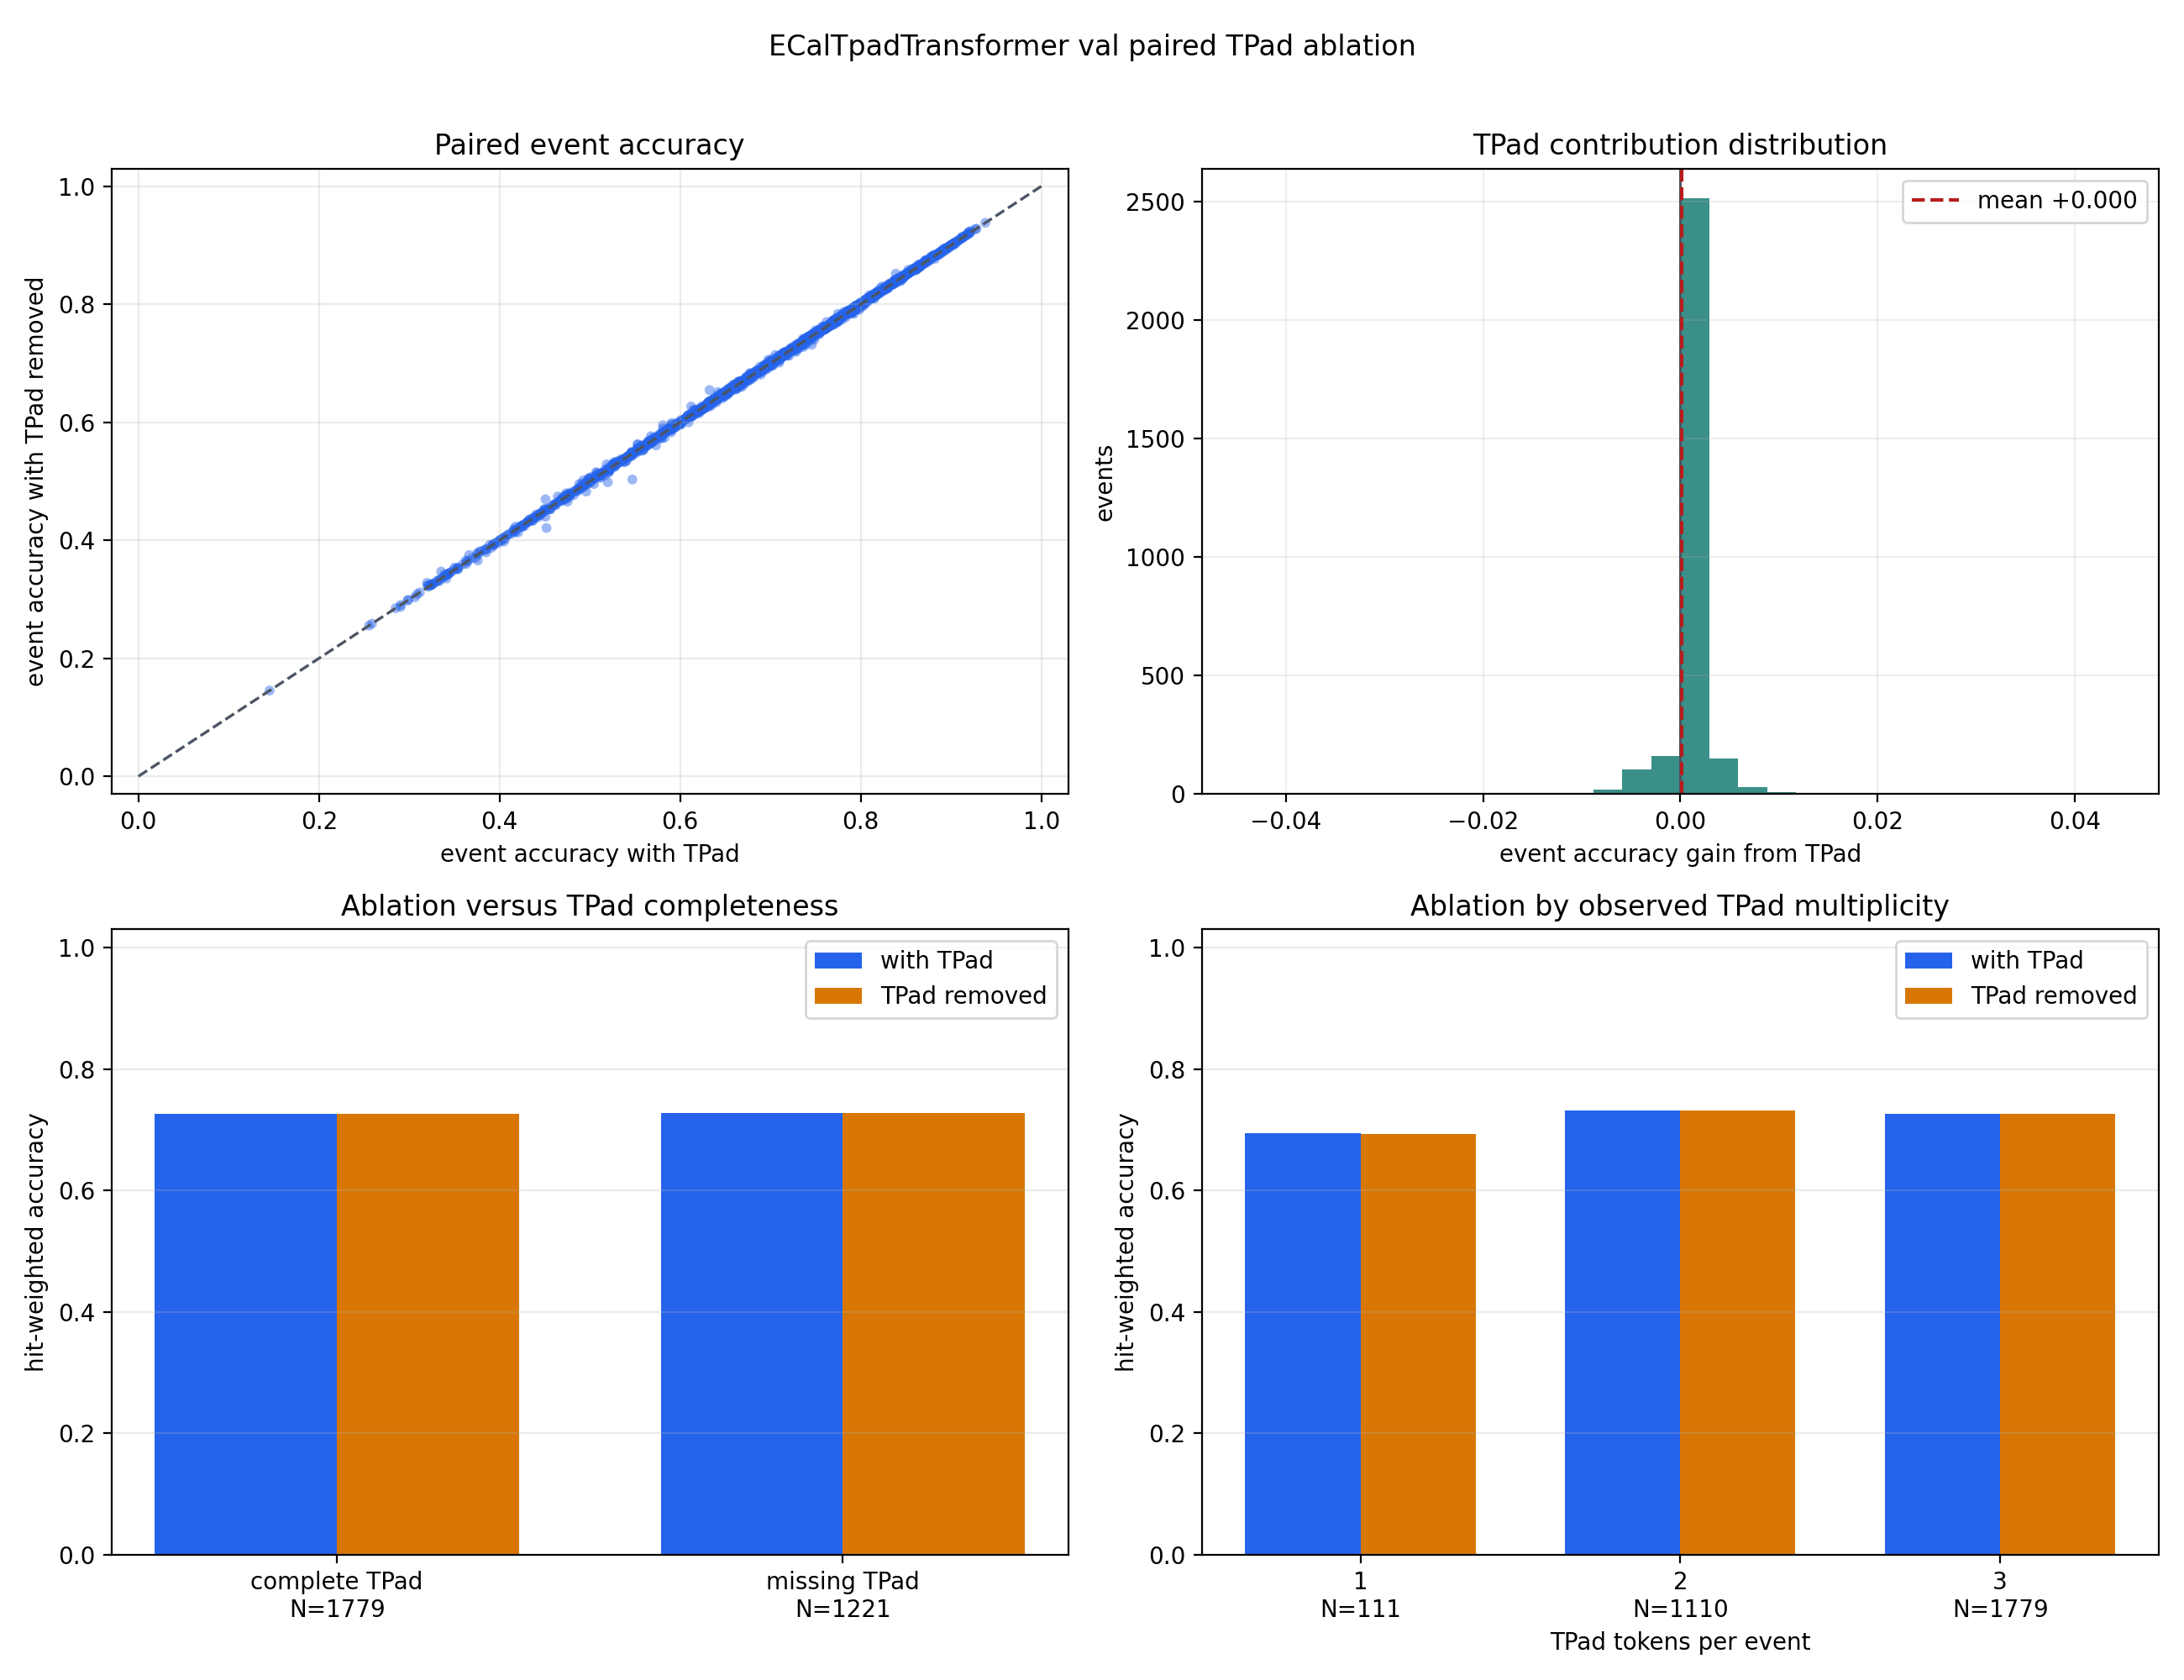
\includegraphics[width=0.98\linewidth]{config/fig/results/tpad_ablation_3e.png}
    \caption{Paired inference-time ablation of trigger-pad-track tokens for a
    trained \(3e\) \texttt{ECalTpadTransformer} on \(3{,}000\) validation
    events. The upper panels compare event accuracy with and without the
    trigger-pad inputs. The lower panels divide the comparison by completeness
    and observed trigger-pad multiplicity.}
    \label{fig:results_tpad_ablation}
\end{figure}

For this trained model and validation sample, the available trigger-pad inputs
therefore have negligible influence on the hit assignments. This is not necessarily a
general conclusion about the information content of the Trigger Scintillator, though it points to that currently.
The plot removes tokens from one already trained model and does not replace a
controlled comparison between separately trained ECal-only and
ECal-plus-trigger-pad models. Techincally, such a comparison is required before the effect
of the additional subdetector input can be stated more broadly, but it will probably not make a difference.

